\section{Appendix}

\subsection{Acknowledgements}

\begin{table}[H]
\centering
\begin{tabular}{|p{0.15\textwidth}|p{0.6\textwidth}|p{0.05\textwidth}|p{0.15\textwidth}|}
\hline
Name           & Use                                                                                   &                                               & Subsystem \\ \hline
Rider          & Primary IDE for development                                                           & \href{https://www.jetbrains.com/rider}{link}                  & DEV       \\ \hline
YouTrack       & Issue tracking software                                                               & \href{https://www.jetbrains.com/youtrack}{link}               & DEV       \\ \hline
VSCode         & Editor used for developing smart contracts                                            & \href{https://code.visualstudio.com}{link}                     & DEV       \\ \hline
RemixIDE       & Web based IDE for developing, testing, deploying and interacting with smart contracts & \href{https://remix.ethereum.org/}{link}                       & DEV       \\ \hline
Azure DevOps   & CD/CI pipeline for running tests and deploying to Azure                               & \href{https://azure.microsoft.com/en-us/services/devops}{link} & DEV       \\ \hline
Azure          & Cloud based deployment                                                                & \href{https://azure.microsoft.com/}{link}                      & DEV       \\ \hline
Ethereum       & Public open source blockchain software with smart contract support                    & \href{https://ethereum.org}{link}                              & BLOCK     \\ \hline
Solidity       & Smart contract programming compiler                                                   & \href{https://docs.soliditylang.org}{link}                     & BLOCK     \\ \hline
Metamask       & Browser extension based Ethereum wallet with over 30 million users                    & \href{https://metamask.io}{link}                               & BLOCK     \\ \hline
Hardhat        & Smart contract development environment                                                & \href{https://hardhat.org}{link}                               & BLOCK     \\ \hline
Waffle         & Smart contract testing framework                                                      & \href{https://getwaffle.io}{link}                              & BLOCK     \\ \hline
ASP.NET        & Web application/service framework for .NET                                            & \href{https://dotnet.microsoft.com/en-us/apps/aspnet}{link}    & BACK-END  \\ \hline
.NET           & Cross platform development framework for C\#                                          & \href{https://dotnet.microsoft.com/en-us/}{link}               & BACK-END  \\ \hline
EFCore         & Object database mapper for .NET                                                       & \href{https://docs.microsoft.com/en-us/ef/core/}{link}         & BACK-END  \\ \hline
Nethereum      & Ethereum interaction library for .NET                                                 & \href{https://nethereum.com/}{link}                            & BACK-END  \\ \hline
NUnit          & .NET test runner                                                                      & \href{https://nunit.org/}{link}                                & BACK-END  \\ \hline
AutoMapper     & .NET object mapping library                                                           & \href{https://automapper.org/}{link}                           & BACK-END  \\ \hline
Cronos         & Cron job handling library                                                             & \href{https://www.nuget.org/packages/Cronos/}{link}            & BACK-END  \\ \hline
iTextSharp     & PDF interaction and modification library used for digital signing                     & \href{https://www.nuget.org/packages/iTextSharp/}{link}        & BACK-END  \\ \hline
TagLibSharp    & Exif tag library used for digital signing                                             & \href{https://github.com/mono/taglib-sharp}{link}              & BACK-END  \\ \hline
ImageSharp     & Image metadata library used for digital signing                                       & \href{https://github.com/SixLabors/ImageSharp}{link}           & BACK-END  \\ \hline
TypeScript     & JavaScript superset providing strong typing                                           & \href{https://www.typescriptlang.org/}{link}                   & FRONT-END \\ \hline
Angular        & JavaScript framework for development of single page dynamic web applications          & \href{https://angular.io/}{link}                               & FRONT-END \\ \hline
Clarity Design & CSS and JavaScript design framework                                                   & \href{https://clarity.design/}{link}                           & FRONT-END \\ \hline
RxJs           & Library for asynchronous JavaScript programming                                       & \href{https://rxjs.dev/}{link}                                 & FRONT-END \\ \hline
Signalr        & Web-socket platform                                                                   & \href{https://www.npmjs.com/package/@microsoft/signalr}{link}  & FRONT-END \\ \hline
web3.js        & Ethereum JavaScript API library                                                       & \href{https://www.npmjs.com/package/web3}{link}                & FRONT-END \\ \hline
\end{tabular}
\end{table}

\subsection{Operational diagrams}

\begin{figure}[H]
\caption{Copyright registration sequence}
\centering
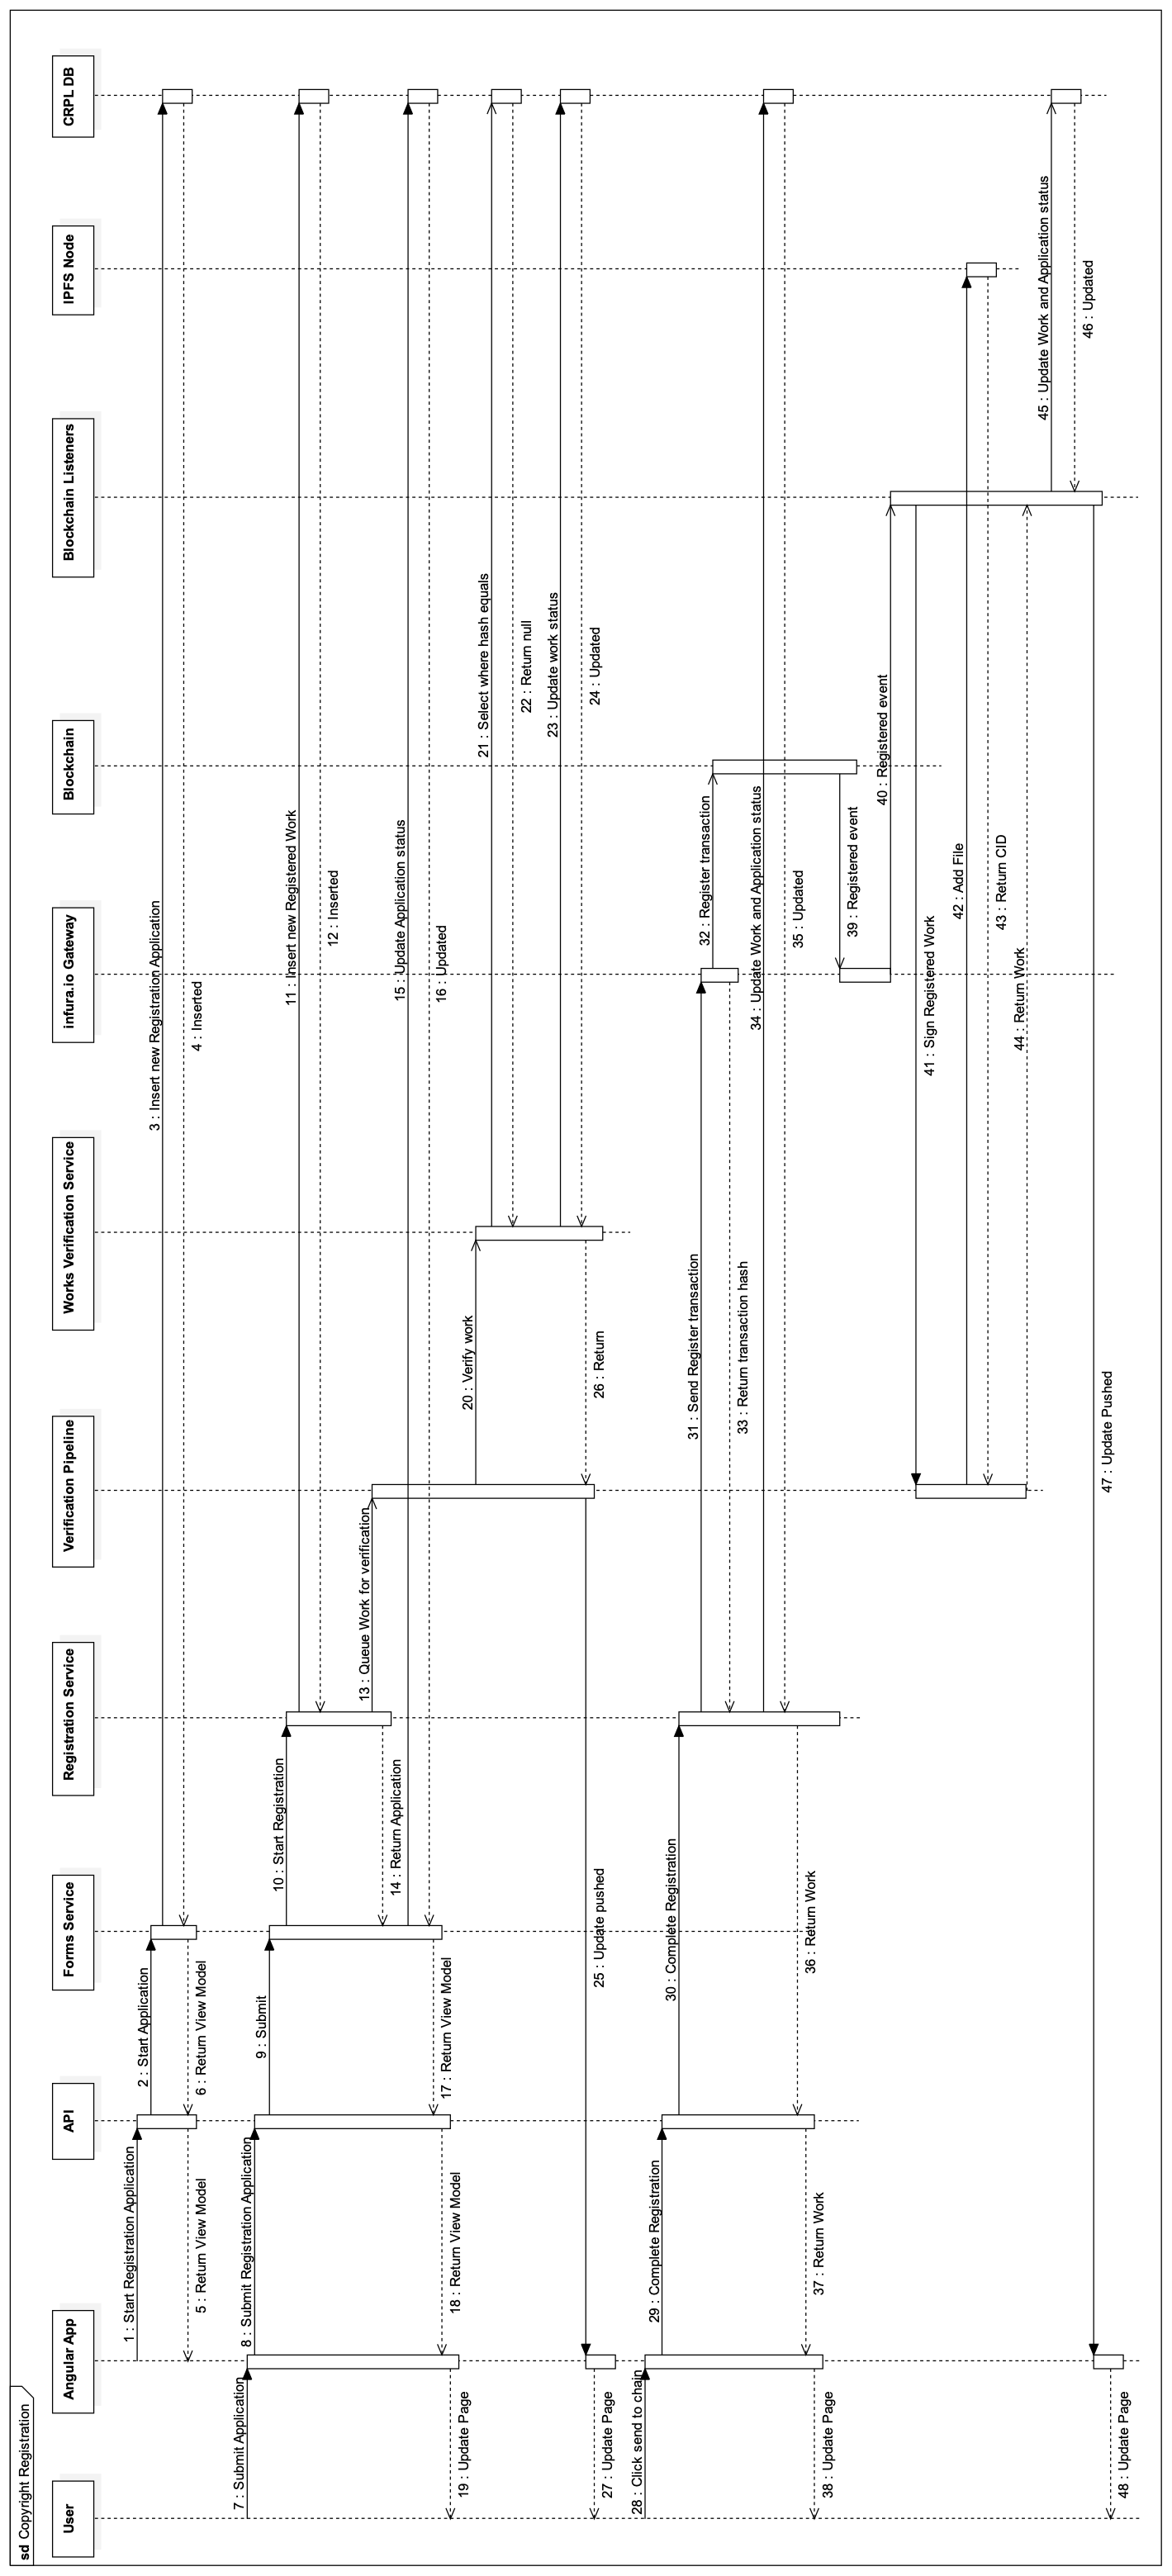
\includegraphics[width=\textwidth,height=0.9\textheight,keepaspectratio]{images/operational/CopyrightRegistration}
\end{figure}

\begin{figure}[H]
\caption{Ownership restructure sequence}
\centering
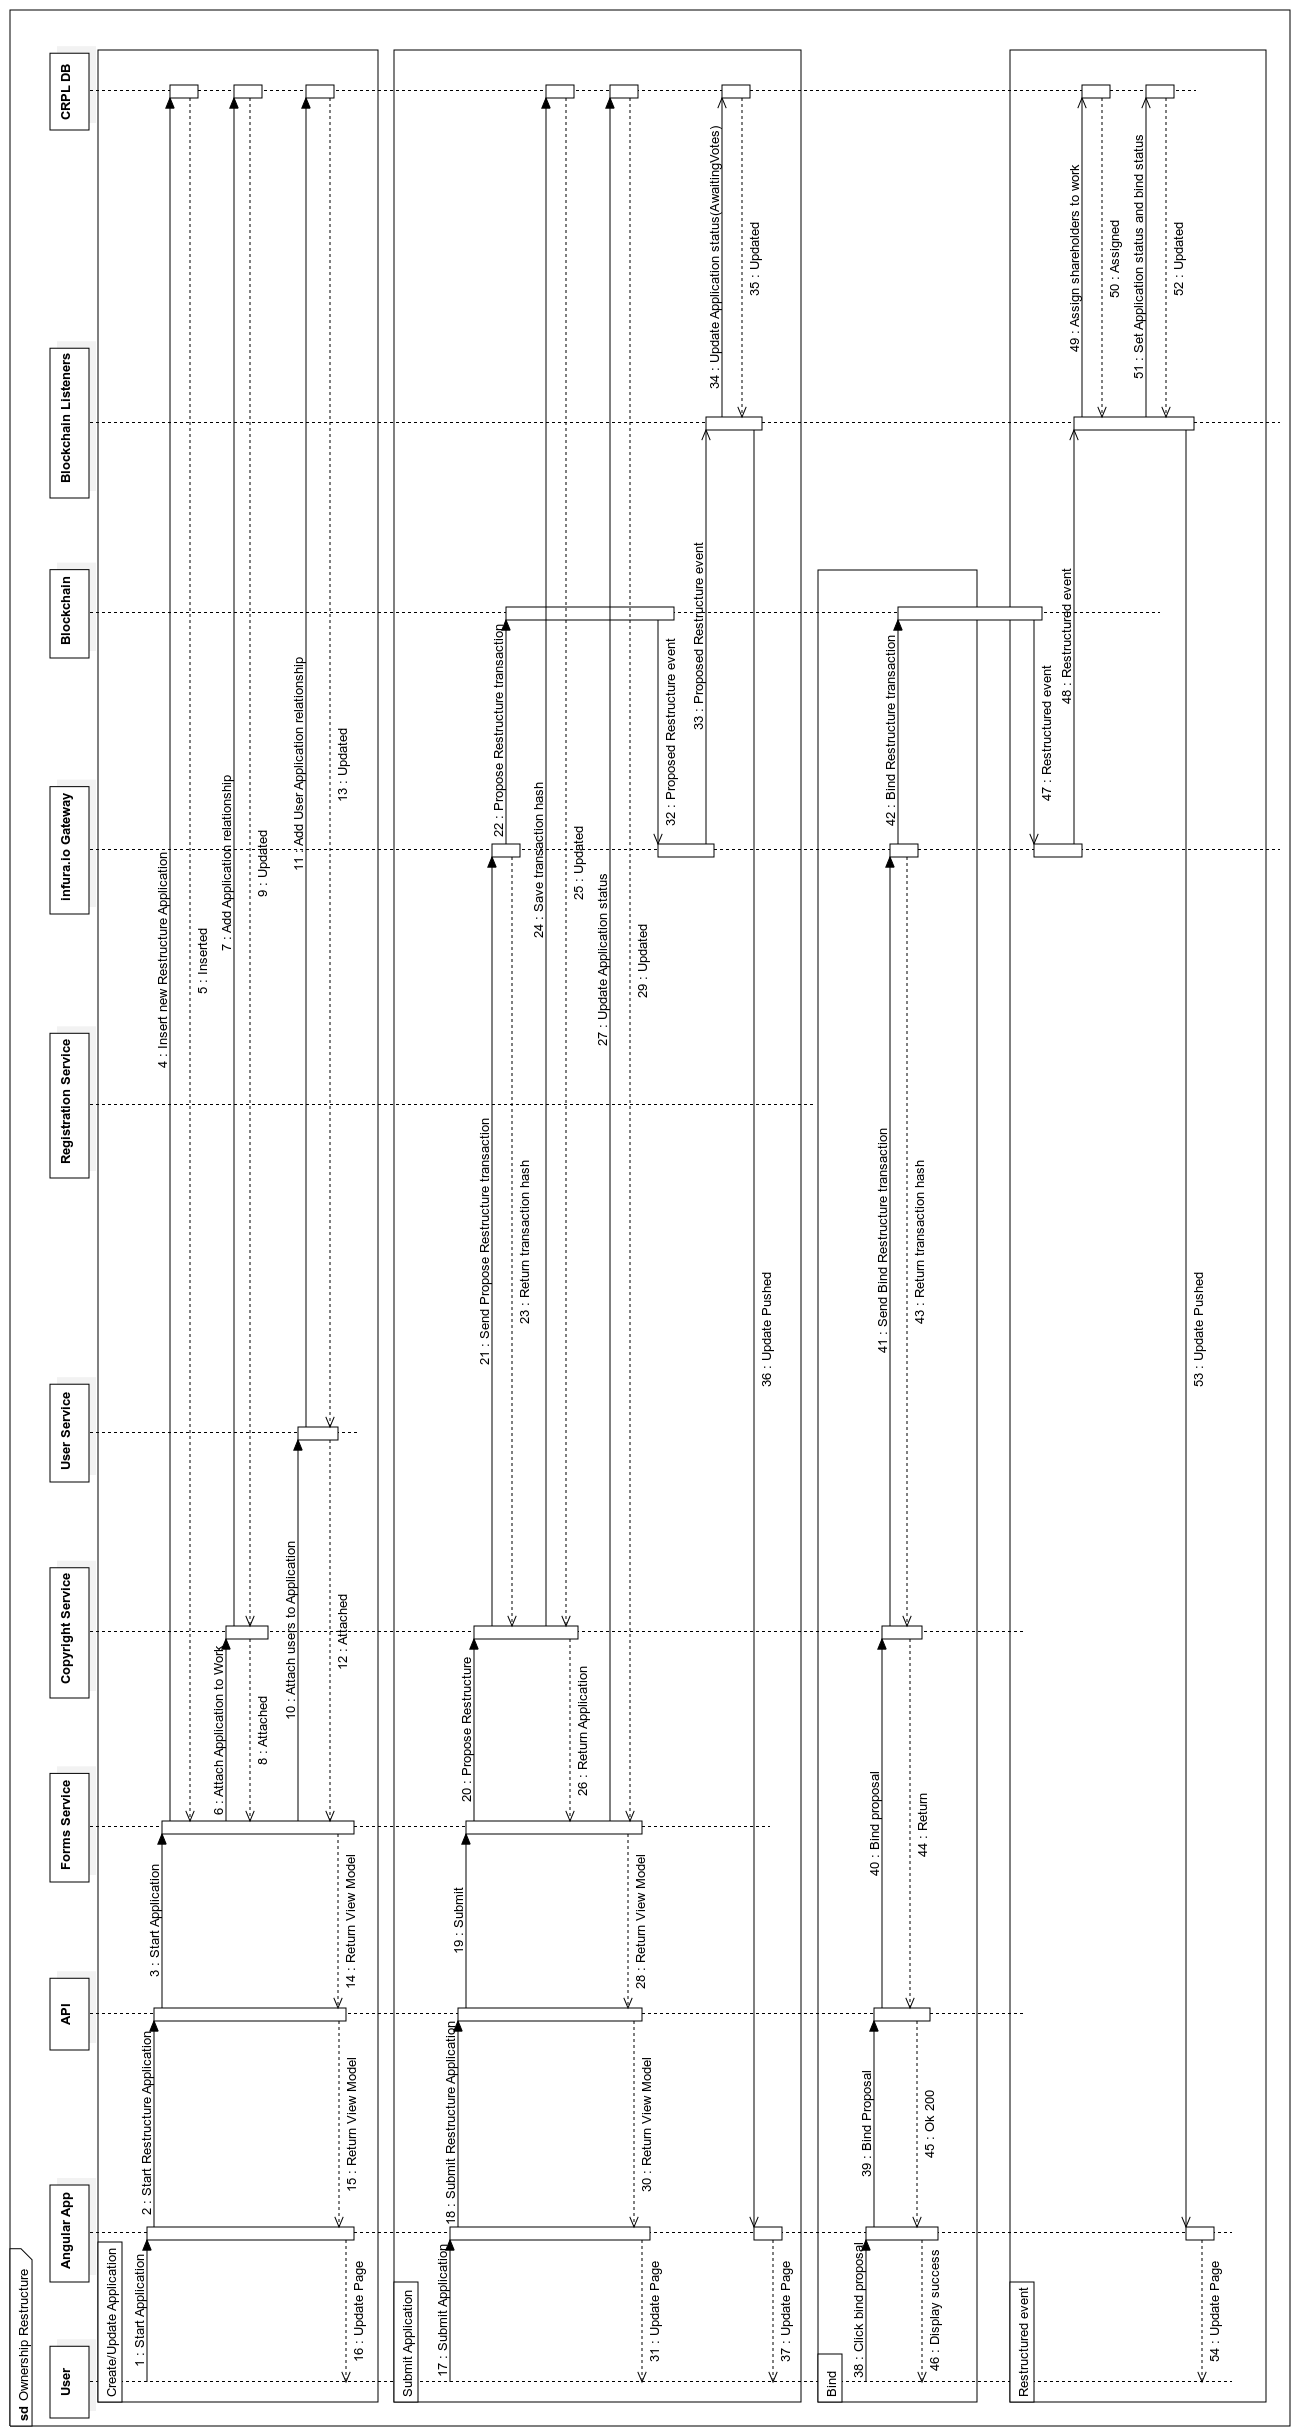
\includegraphics[width=\textwidth,height=\textheight,keepaspectratio]{images/operational/OwnershipRestructure}
\end{figure}

\begin{figure}[H]
\caption{Dispute with payment expected recourse sequence}
\centering
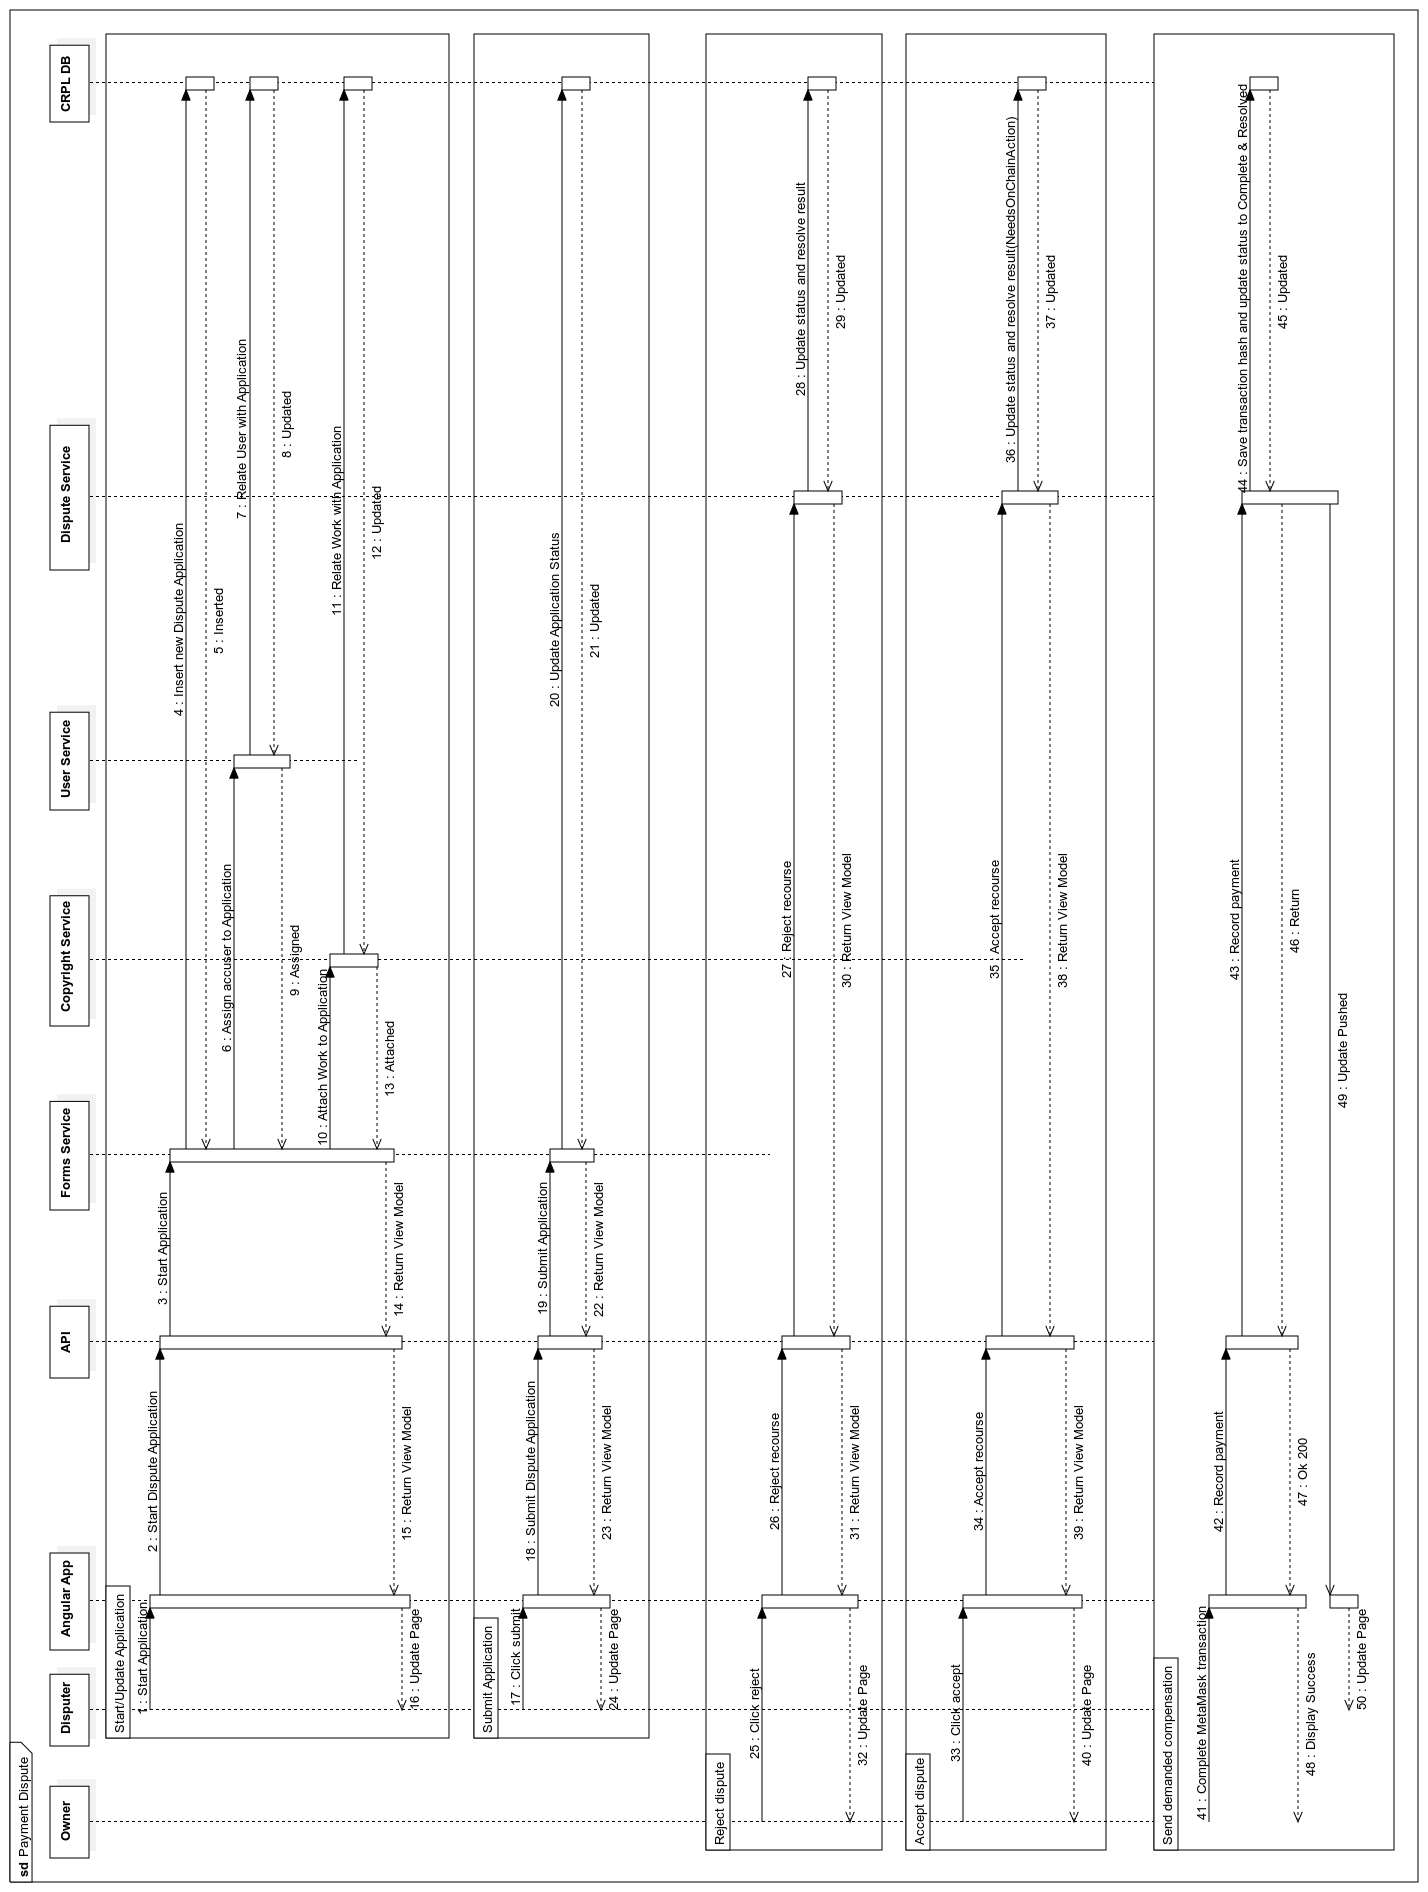
\includegraphics[width=\textwidth,height=\textheight,keepaspectratio]{images/operational/PaymentDispute}
\end{figure}

\begin{figure}[H]
\caption{User Authentication (Login/Create Account) sequence}
\centering
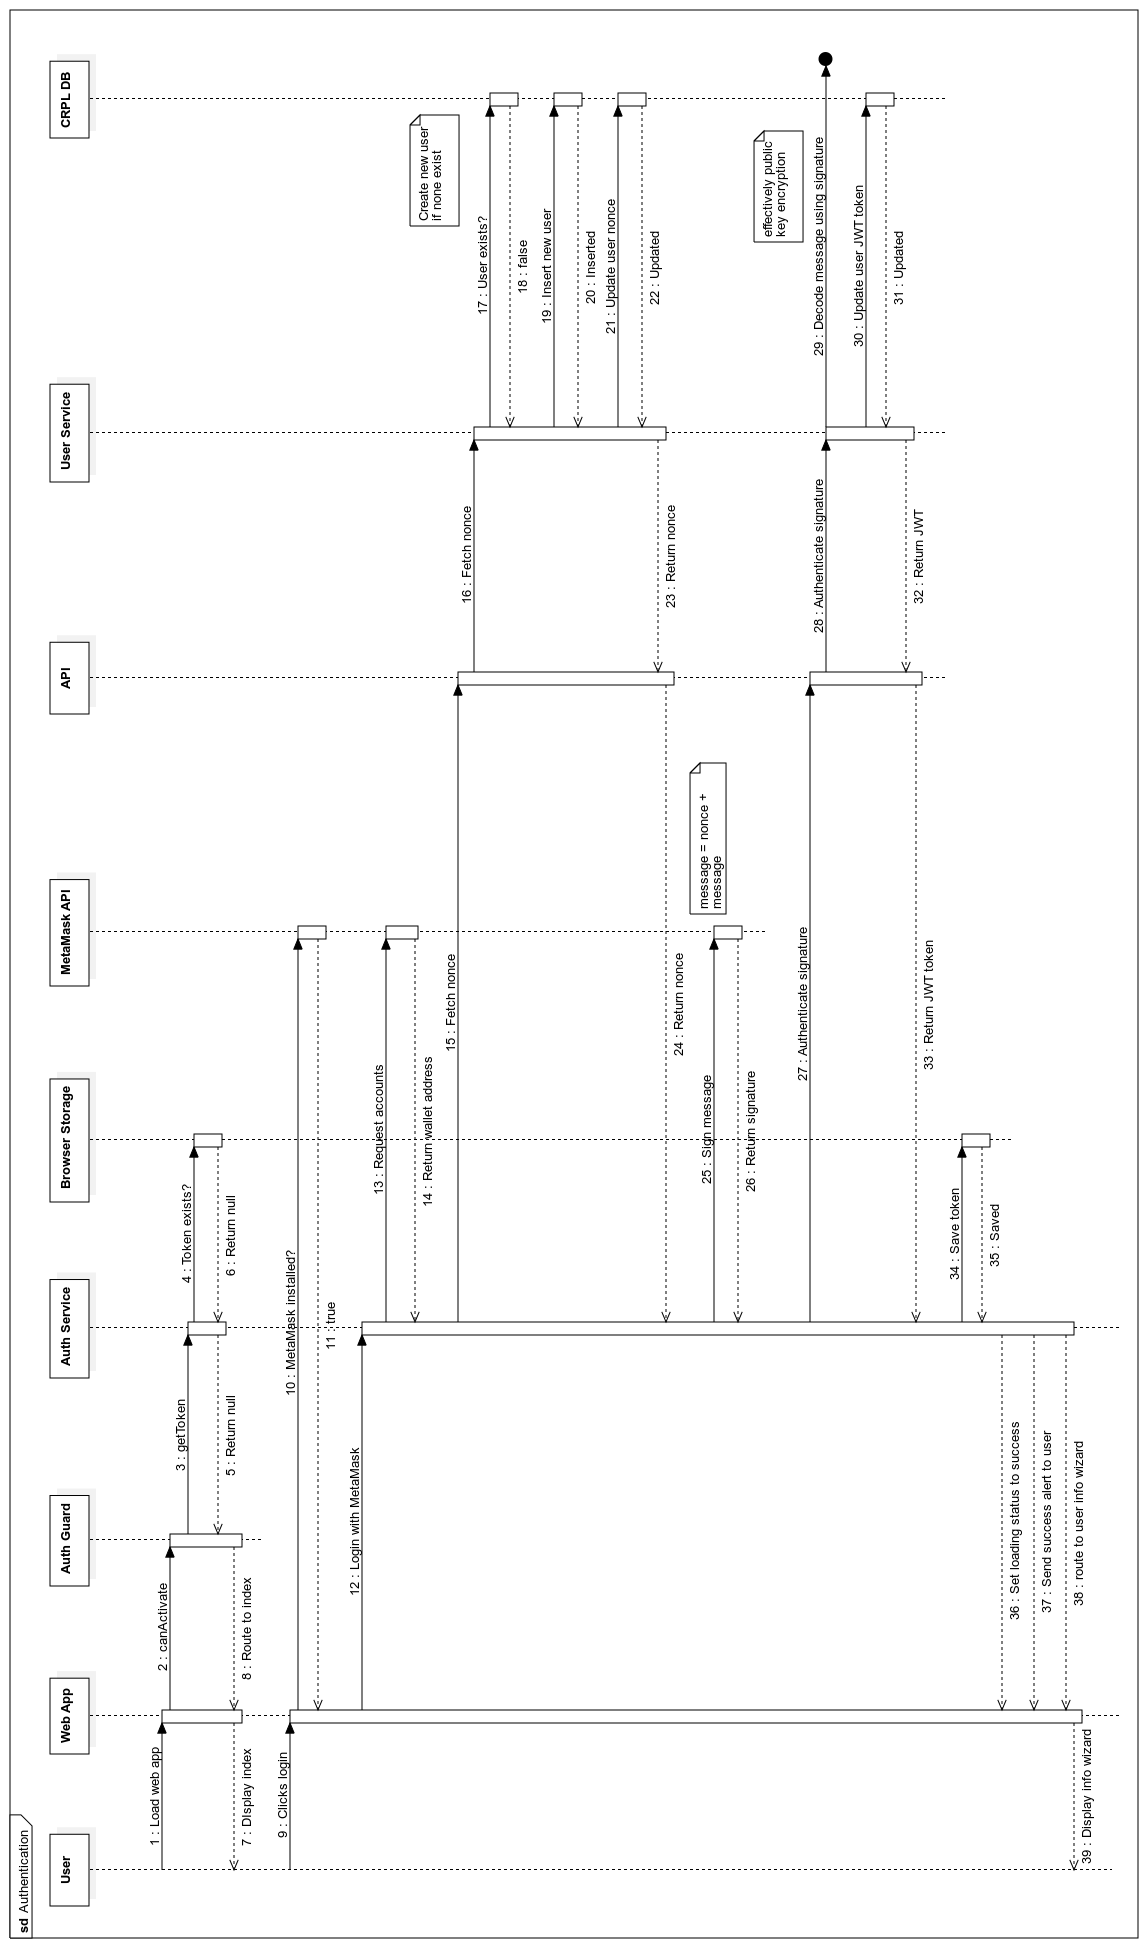
\includegraphics[width=\textwidth,height=\textheight,keepaspectratio]{images/operational/Authentication}
\end{figure}

\begin{figure}[H]
\caption{Angular Guarding of pages sequence}
\centering
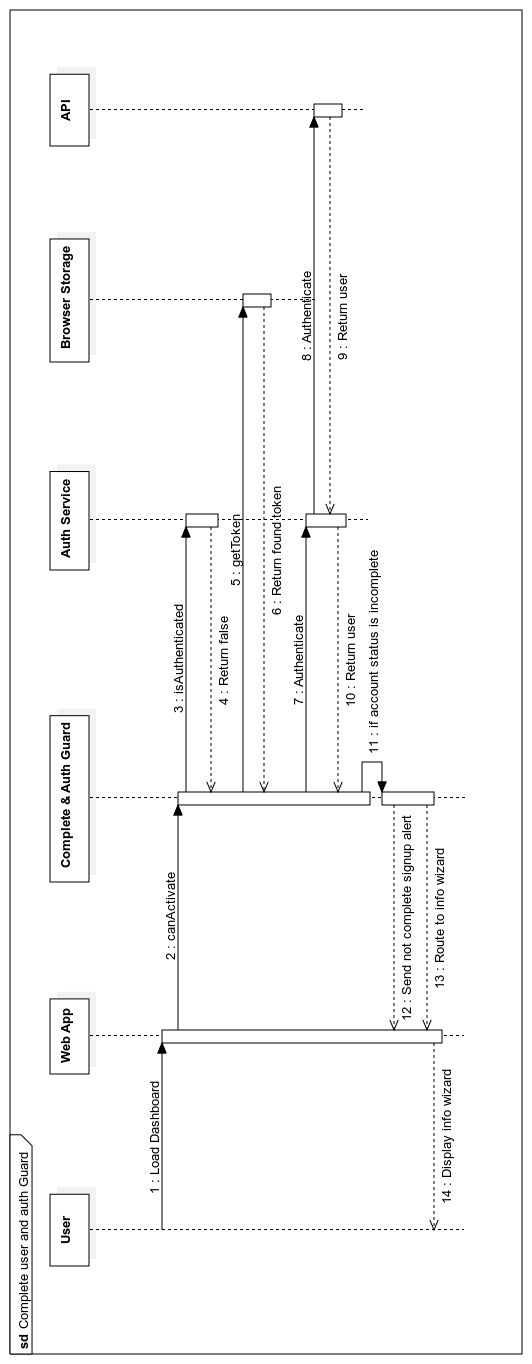
\includegraphics[width=\textwidth,height=\textheight,keepaspectratio]{images/operational/Guard}
\end{figure}

\begin{figure}[H]
\caption{Blockchain event processing sequence}
\centering
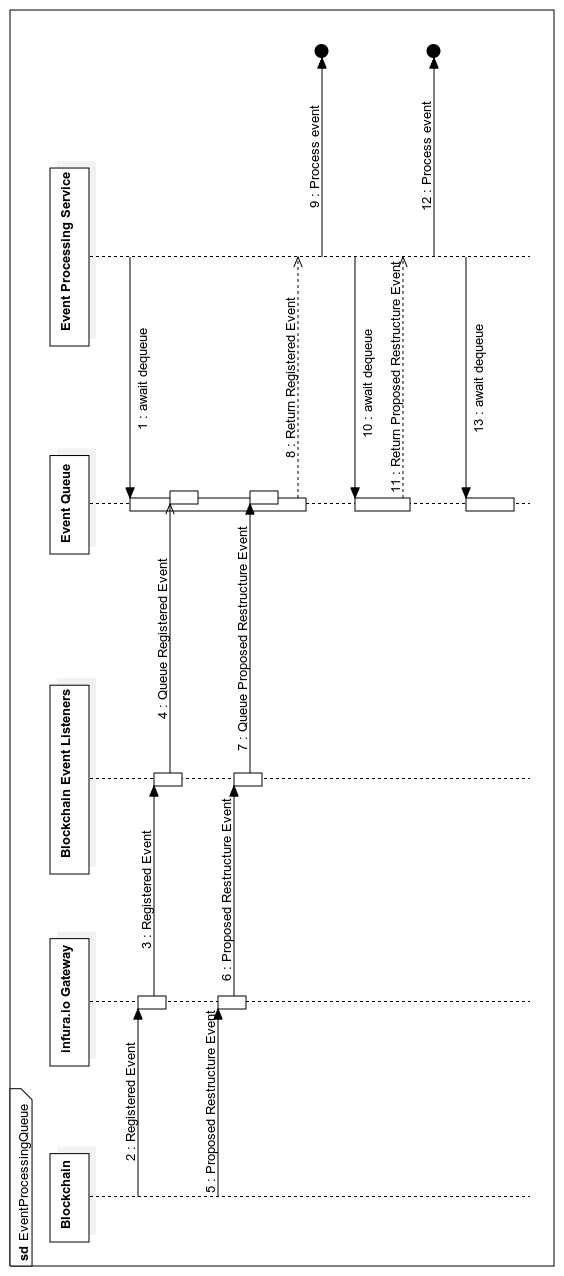
\includegraphics[width=\textwidth,height=\textheight,keepaspectratio]{images/operational/EventProcessingQueue}
\end{figure}

\begin{figure}[H]
\caption{Smart contract Register function flowchart}
\centering
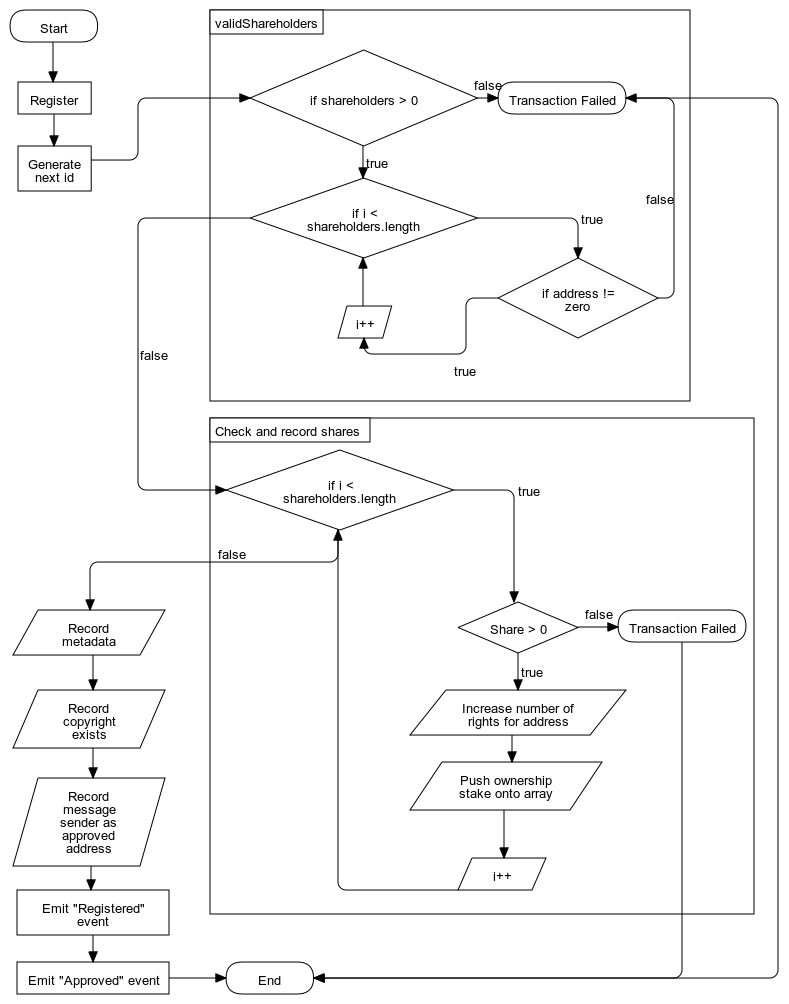
\includegraphics[width=\textwidth,height=\textheight,keepaspectratio]{images/operational/Register}
\end{figure}

\begin{figure}[H]
\caption{Resonance service (WebSocket service) sequence}
\centering
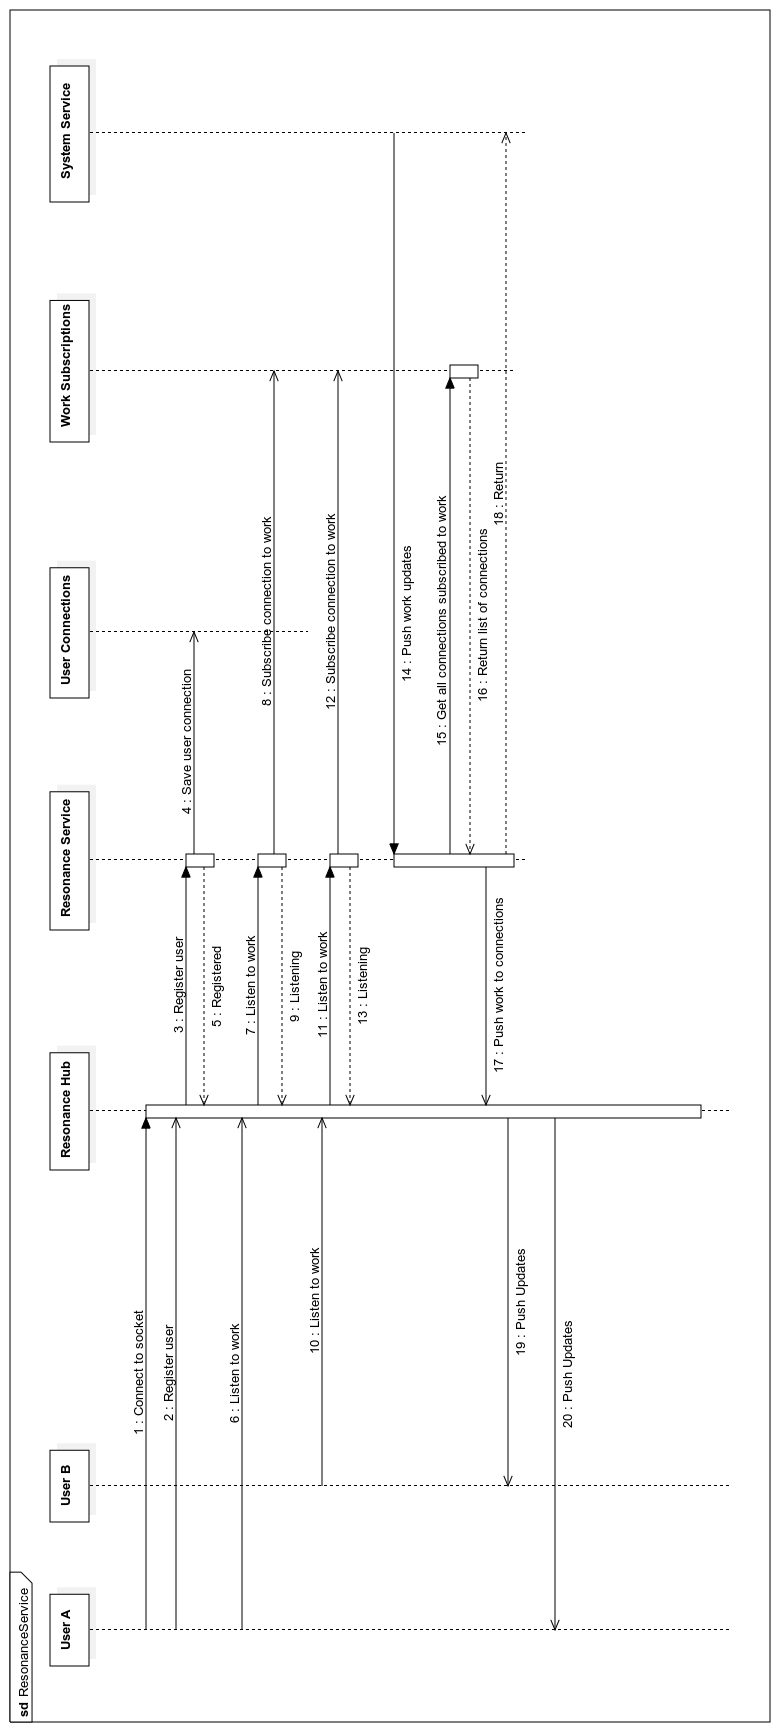
\includegraphics[width=\textwidth,height=\textheight,keepaspectratio]{images/operational/ResonanceService}
\end{figure}

\subsection{Design docs}

\begin{figure}[H]
\caption{Original index page wireframe}
\centering
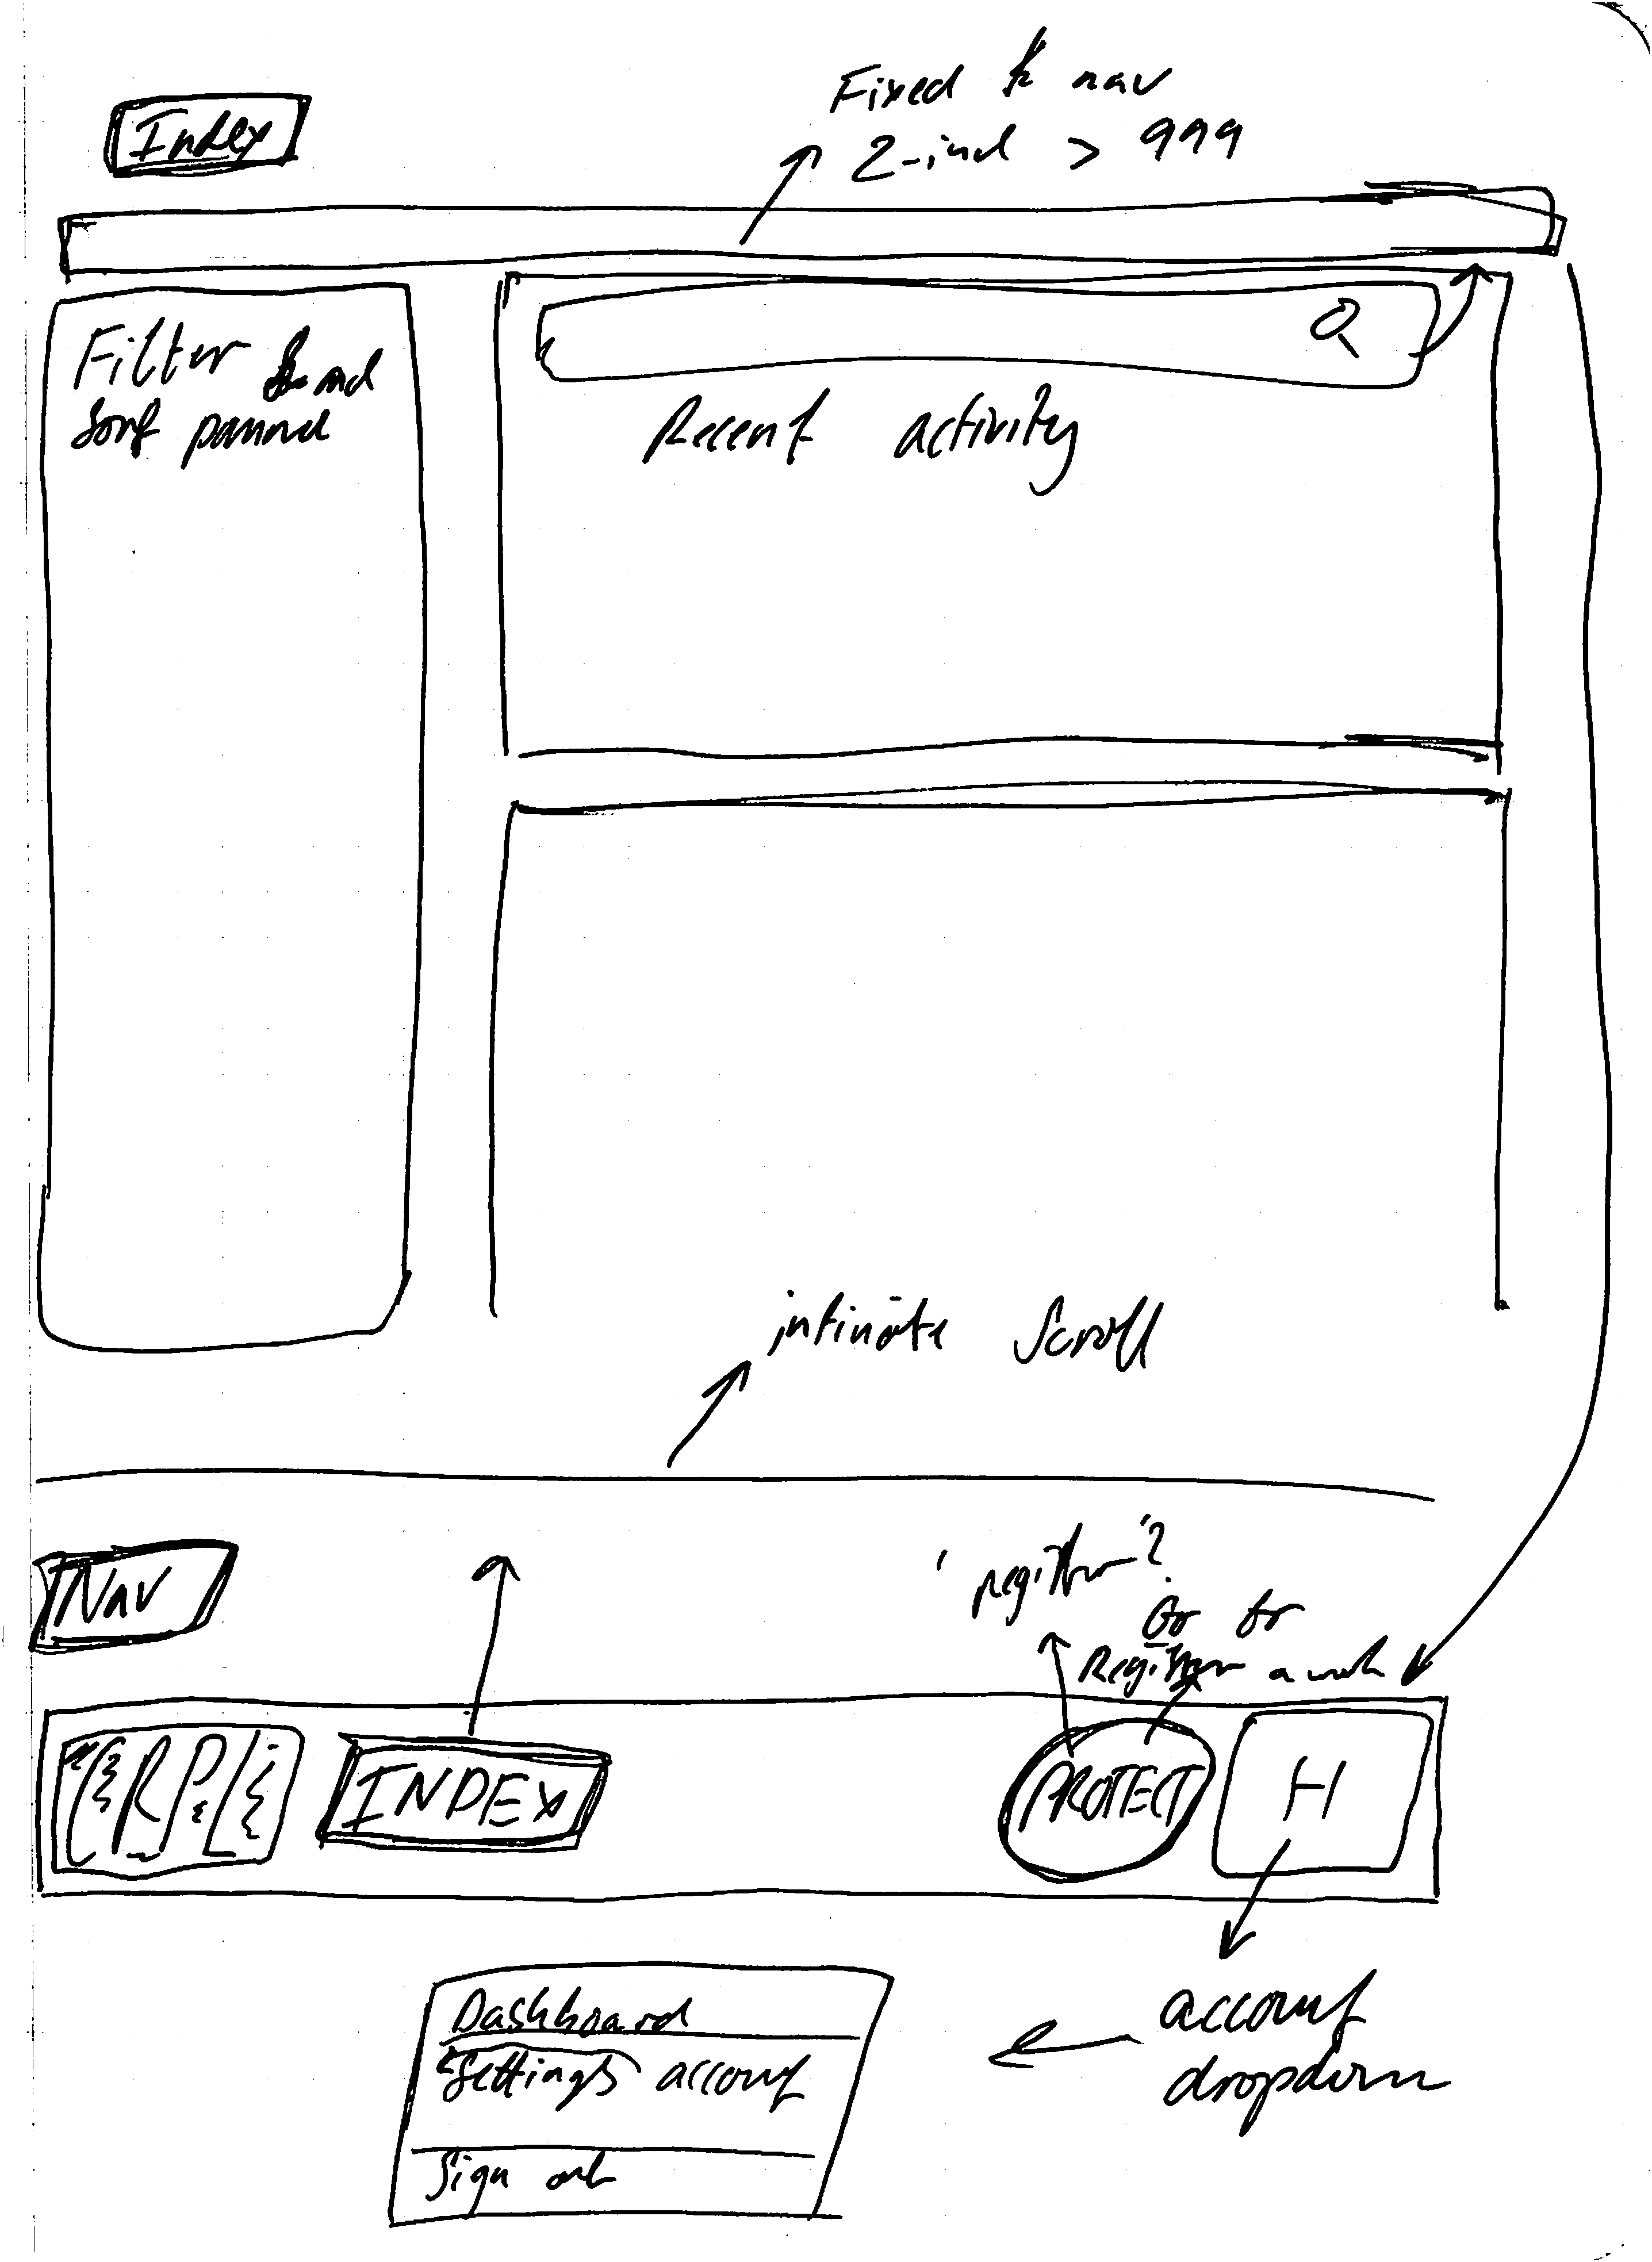
\includegraphics[width=0.7\textwidth,height=\textheight,keepaspectratio]{images/appendix/design/docs/index}
\end{figure}

\begin{figure}[H]
\caption{Original dashboard page wireframe}
\centering
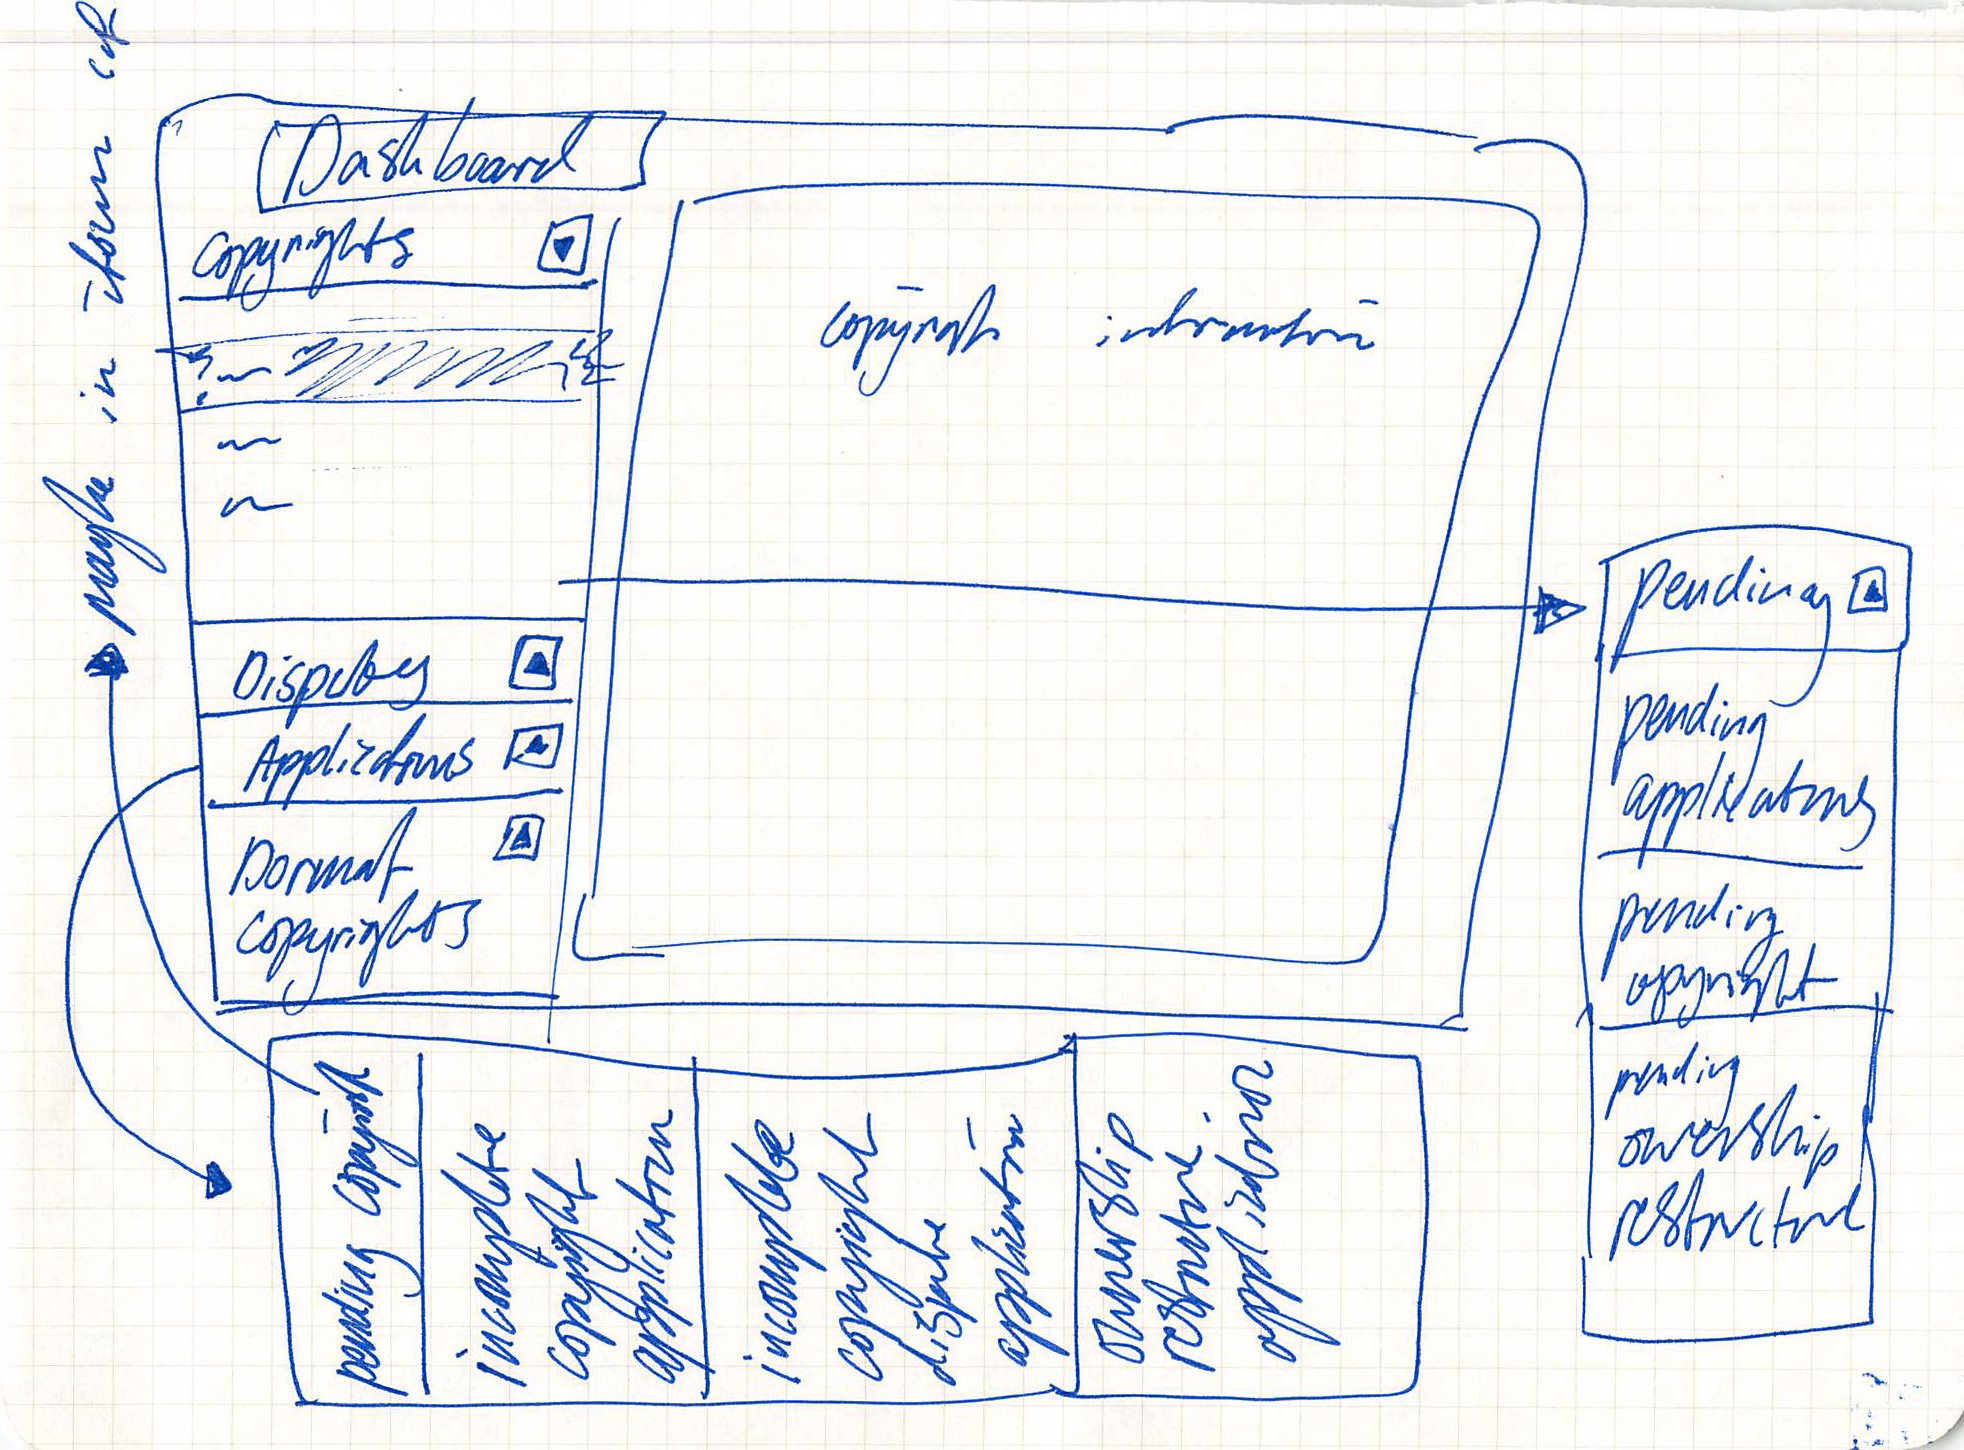
\includegraphics[width=0.8\textwidth,height=\textheight,keepaspectratio]{images/appendix/design/docs/dash}
\end{figure}

\begin{figure}[H]
\caption{Early system architecture diagram}
\centering
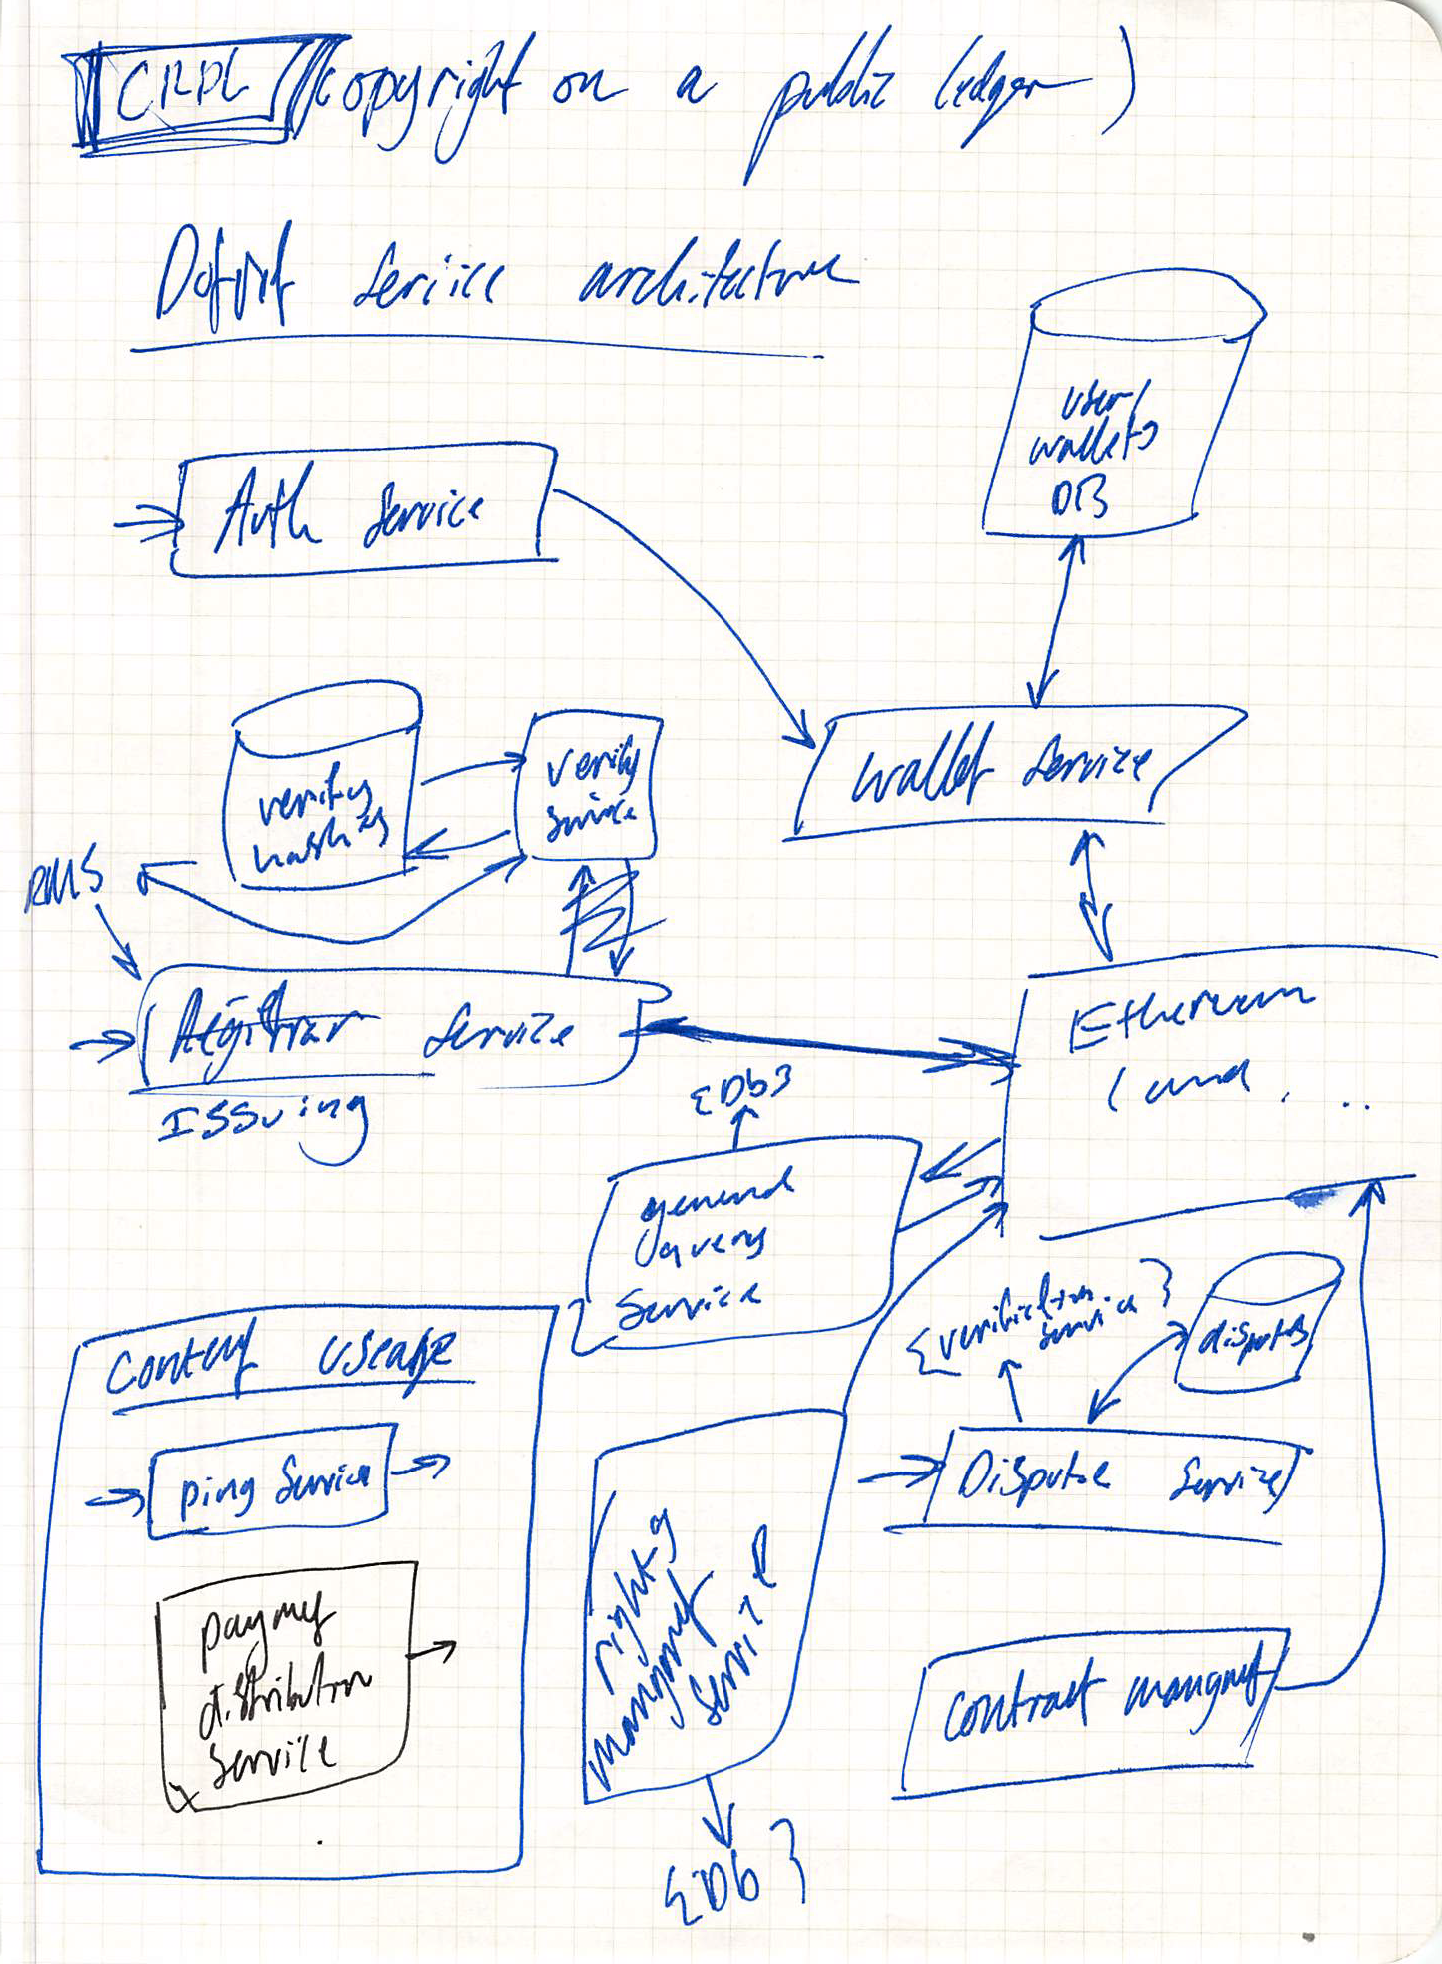
\includegraphics[width=0.7\textwidth,height=\textheight,keepaspectratio]{images/appendix/design/docs/arch}
\end{figure}

\begin{figure}[H]
\caption{Copyright registration state flow diagram}
\centering
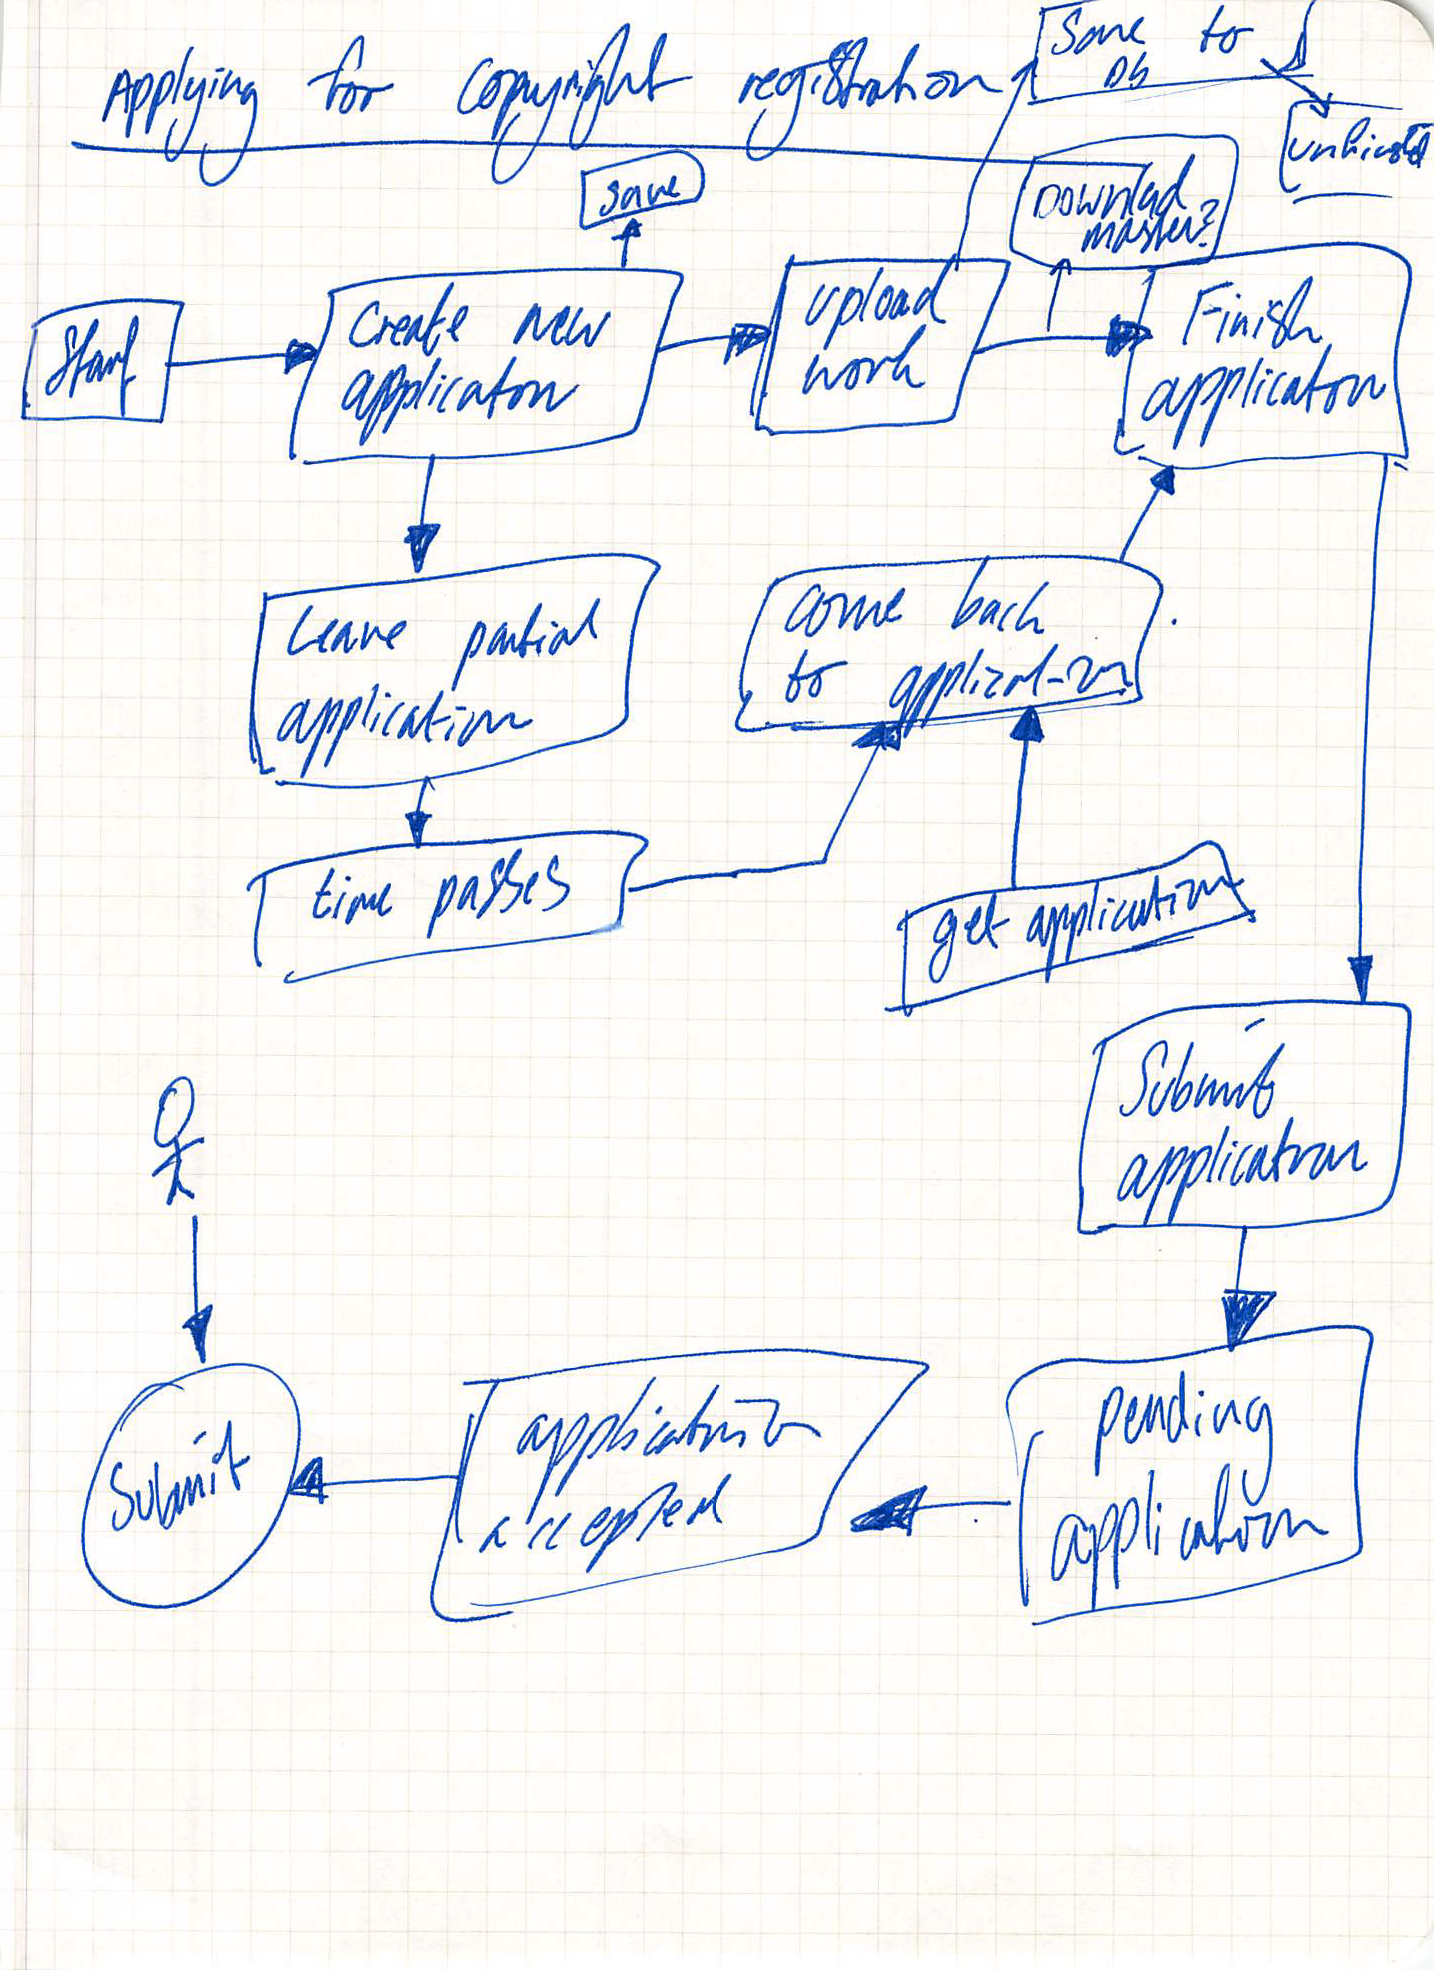
\includegraphics[width=0.7\textwidth,height=\textheight,keepaspectratio]{images/appendix/design/docs/reg}
\end{figure}

\begin{figure}[H]
\caption{Ownership restructure state flow diagram}
\centering
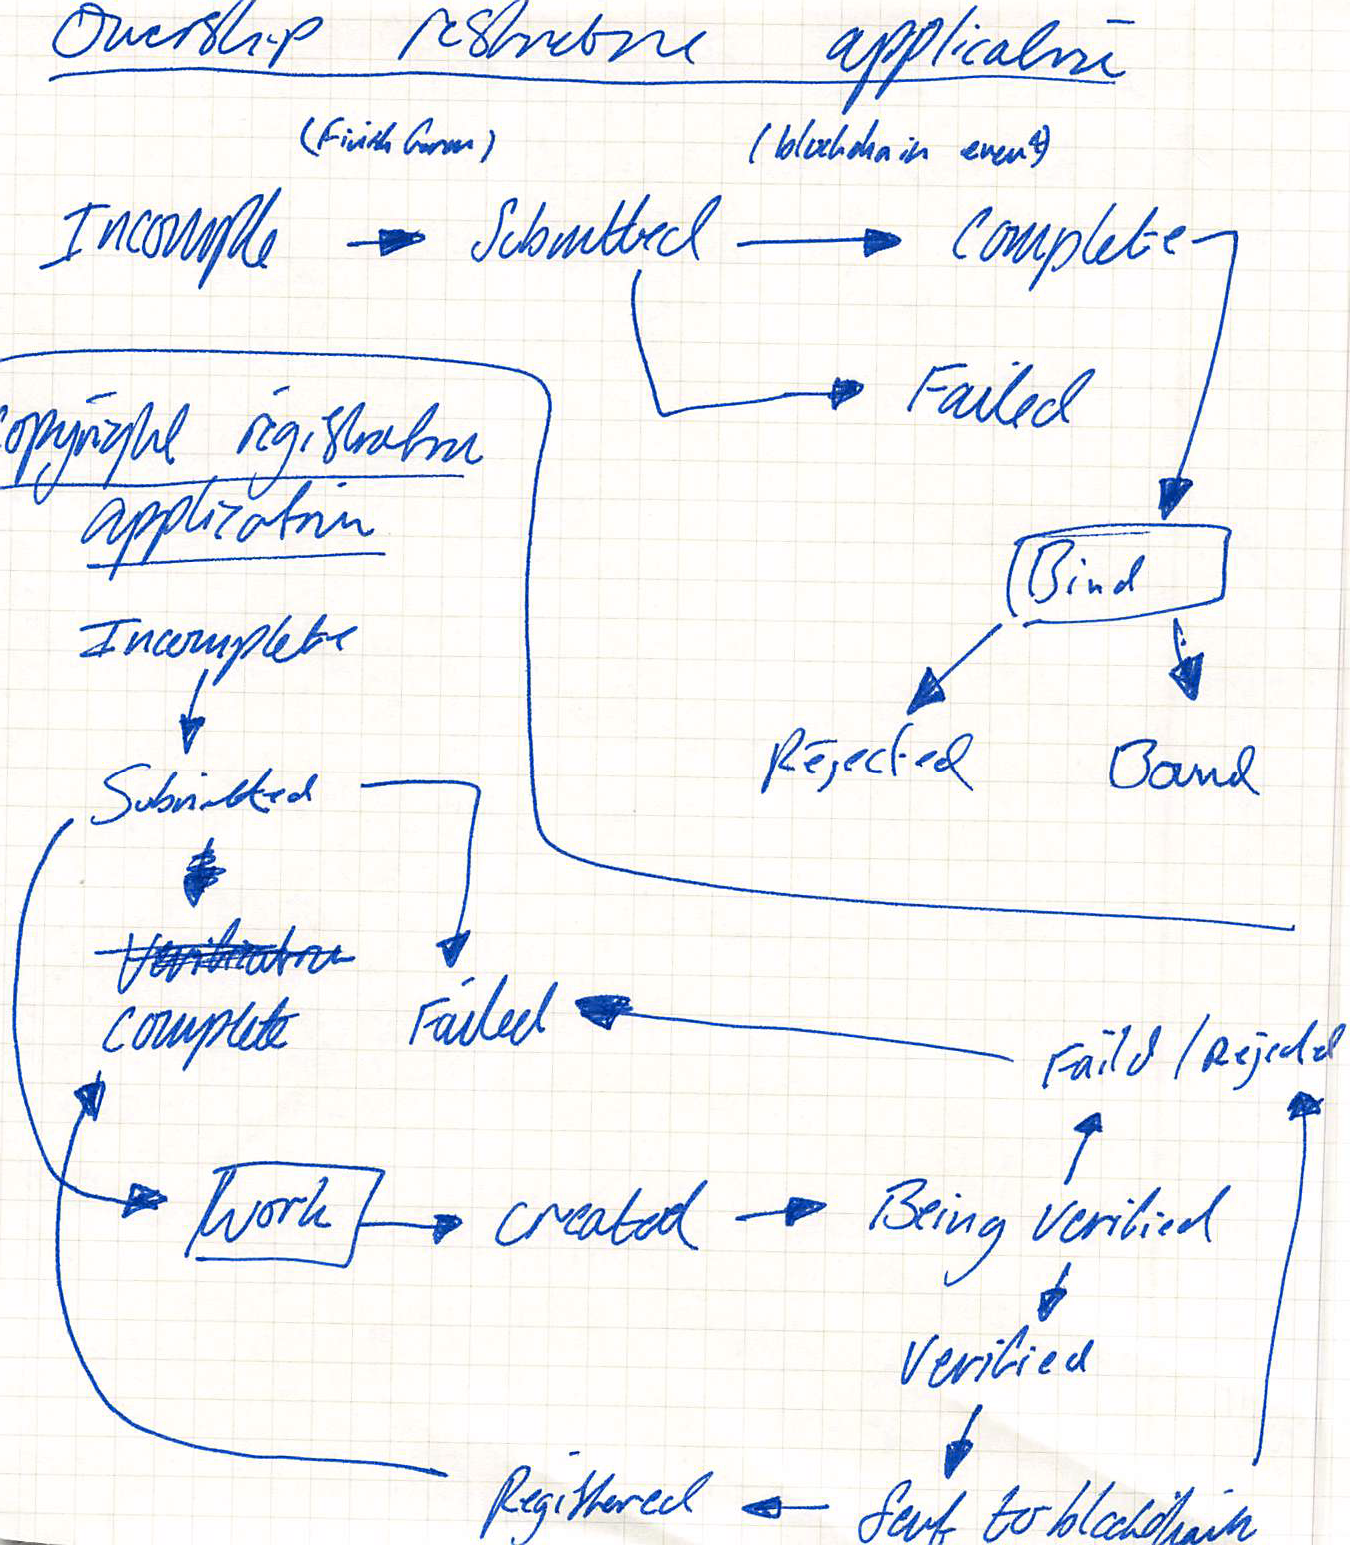
\includegraphics[width=0.7\textwidth,height=\textheight,keepaspectratio]{images/appendix/design/docs/restruct}
\end{figure}

\begin{figure}[H]
\caption{Original dispute handling flow diagram}
\centering
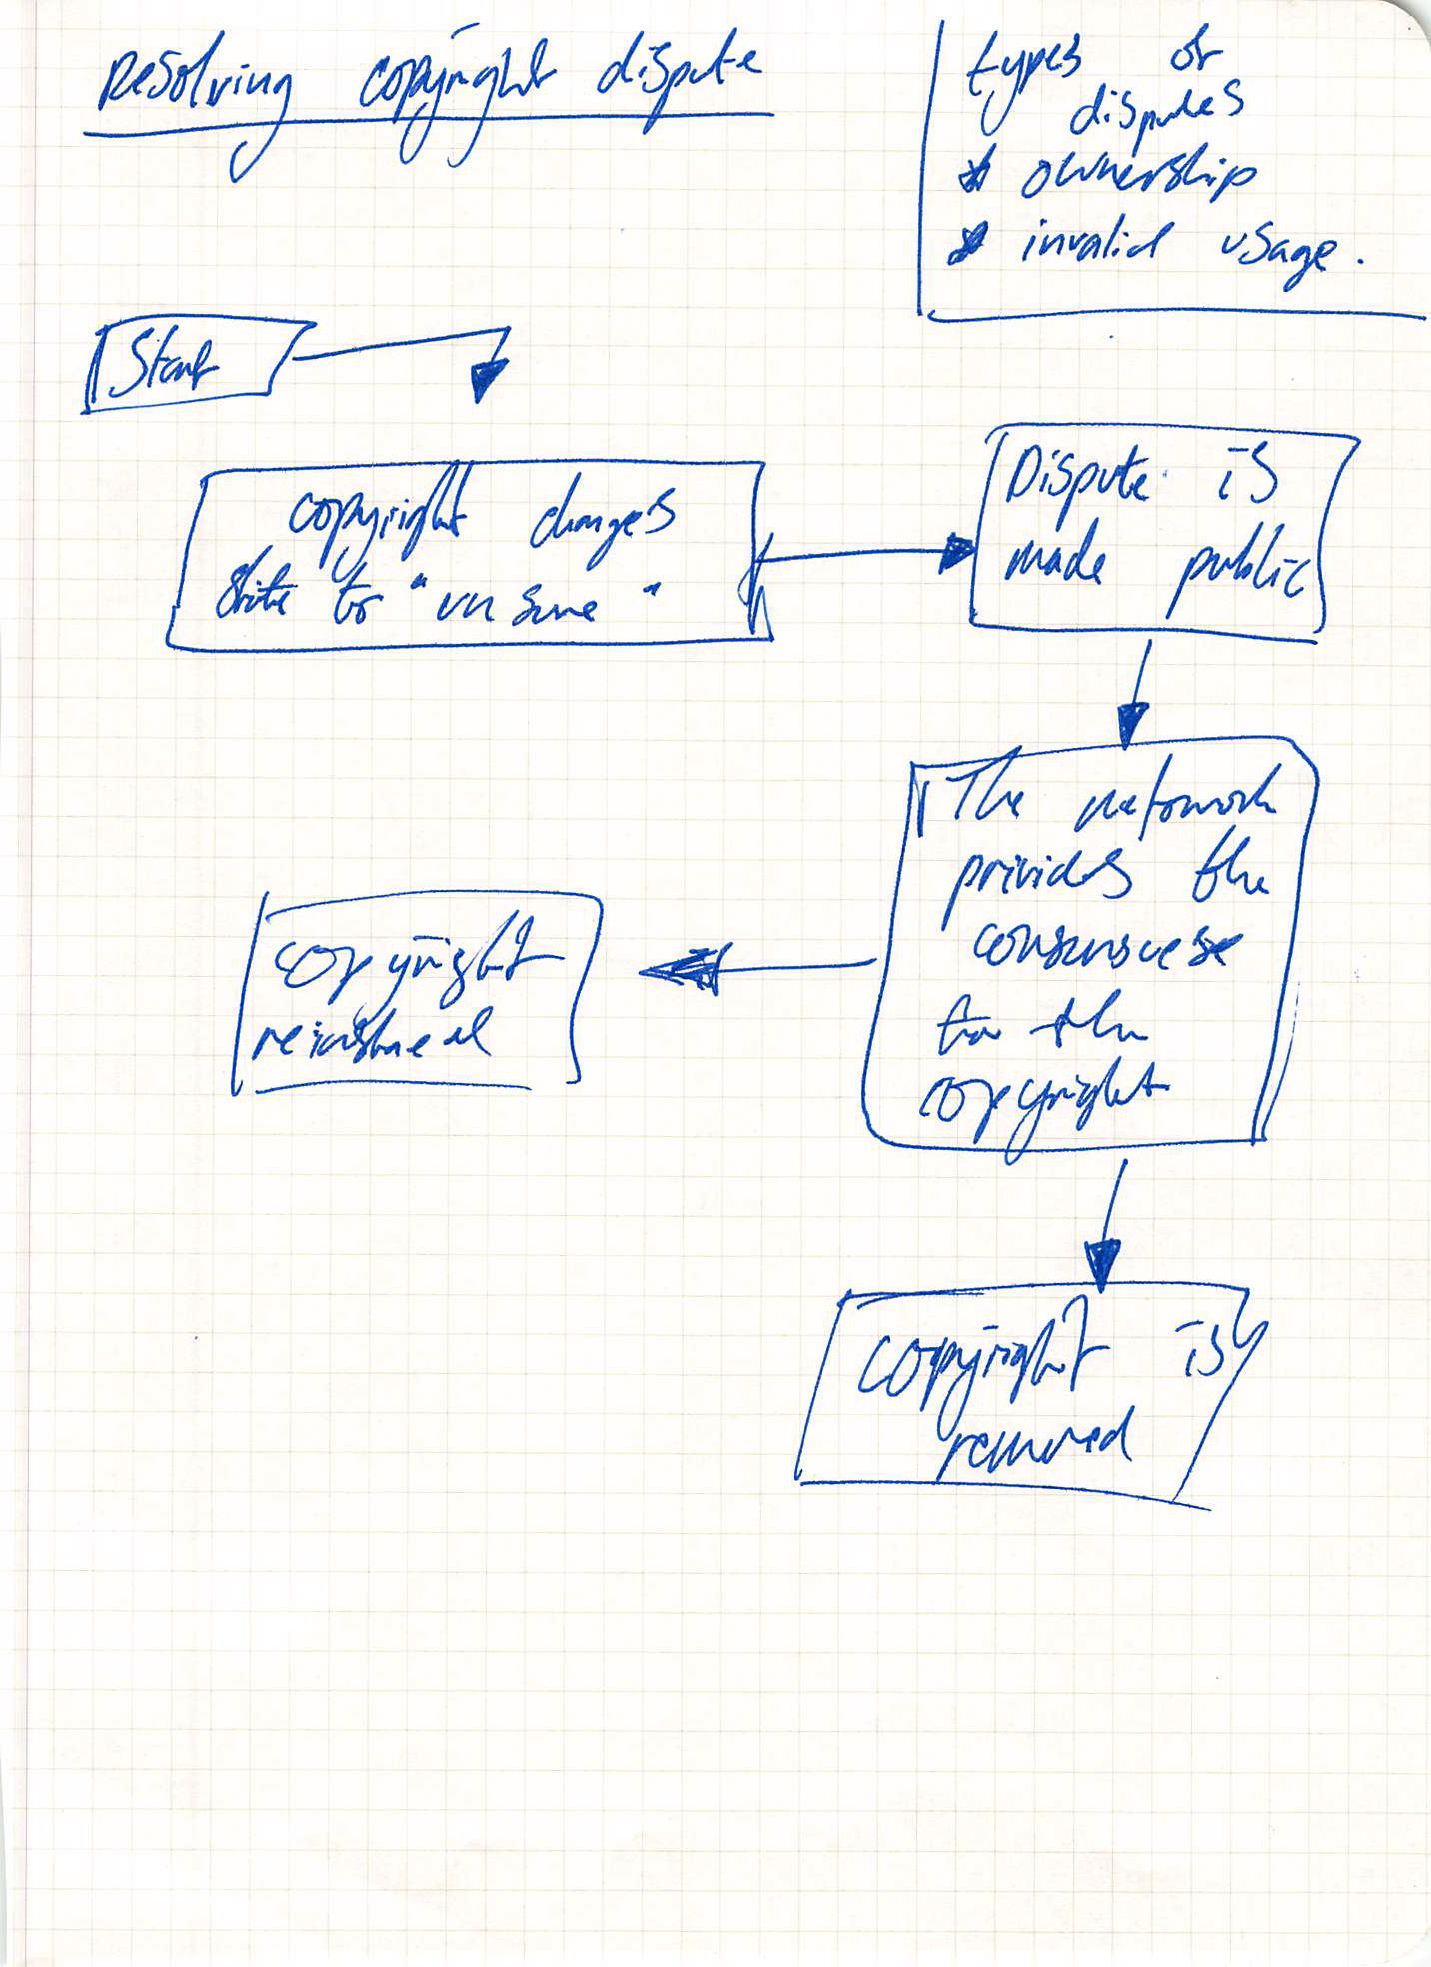
\includegraphics[width=0.7\textwidth,height=\textheight,keepaspectratio]{images/appendix/design/docs/dispute}
\end{figure}

\begin{figure}[H]
\caption{Original blockchain event listening diagram}
\centering
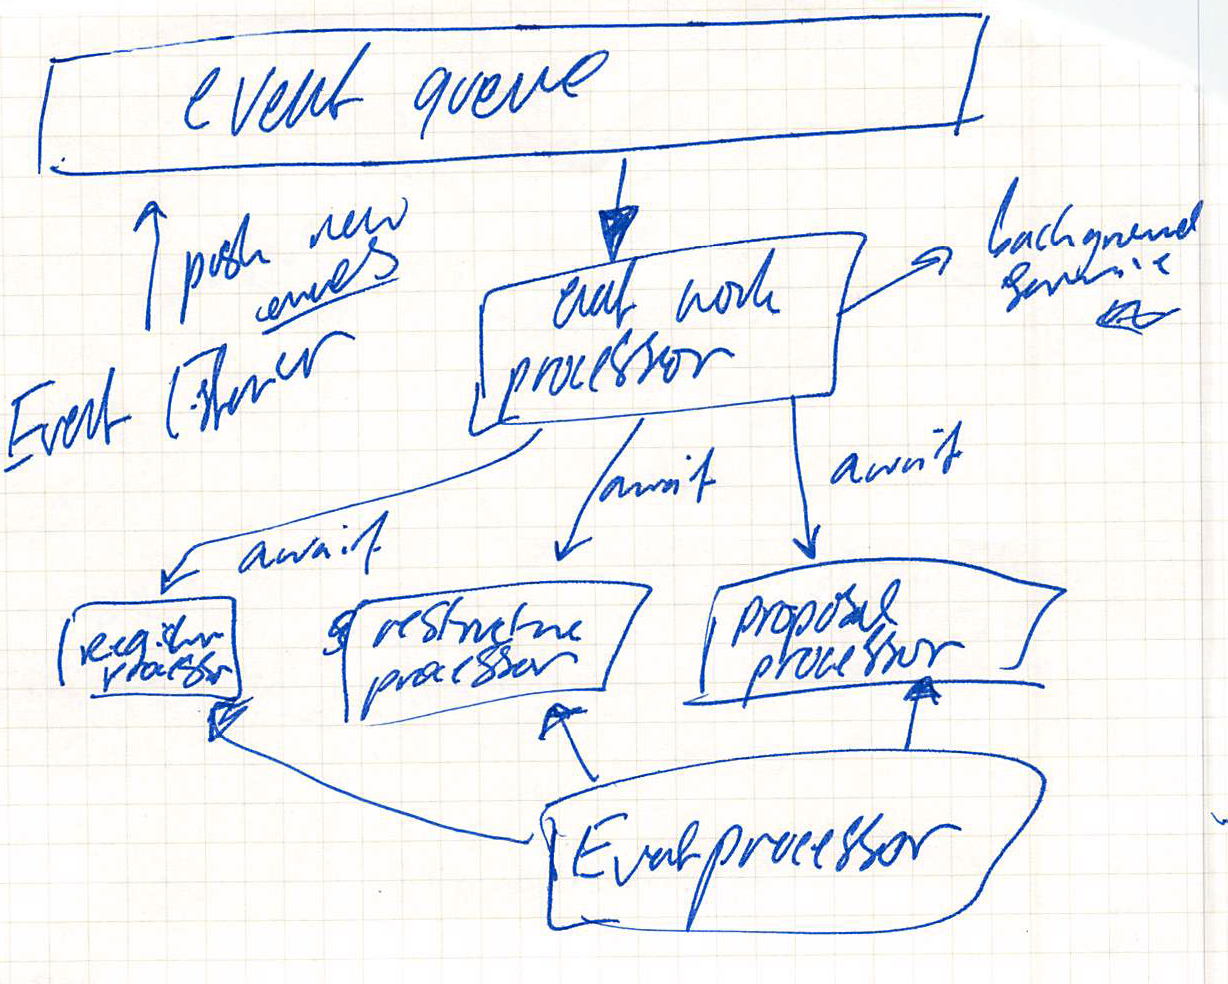
\includegraphics[width=0.7\textwidth,height=\textheight,keepaspectratio]{images/appendix/design/docs/event}
\end{figure}

\subsection{Sprint reviews}

Sprint reviews can also be found on the \href{https://github.com/mrharrisonbarker/crpl#readme}{README}.

\includepdf[pages=-]{./images/appendix/SprintReviews.pdf}

\subsection{User guide}

The user guide can be found at \href{https://github.com/MrHarrisonBarker/CRPL/wiki}{https://github.com/MrHarrisonBarker/CRPL/wiki}

If you want to run this software locally on your machine then I would strongly suggest following my instructions on the \href{https://github.com/MrHarrisonBarker/CRPL#readme}{README} for installation and running.

\subsection{Test results}
\label{sec:test-results}

\subsubsection{Smart contract unit test results}
\label{sec:test-results:smart}

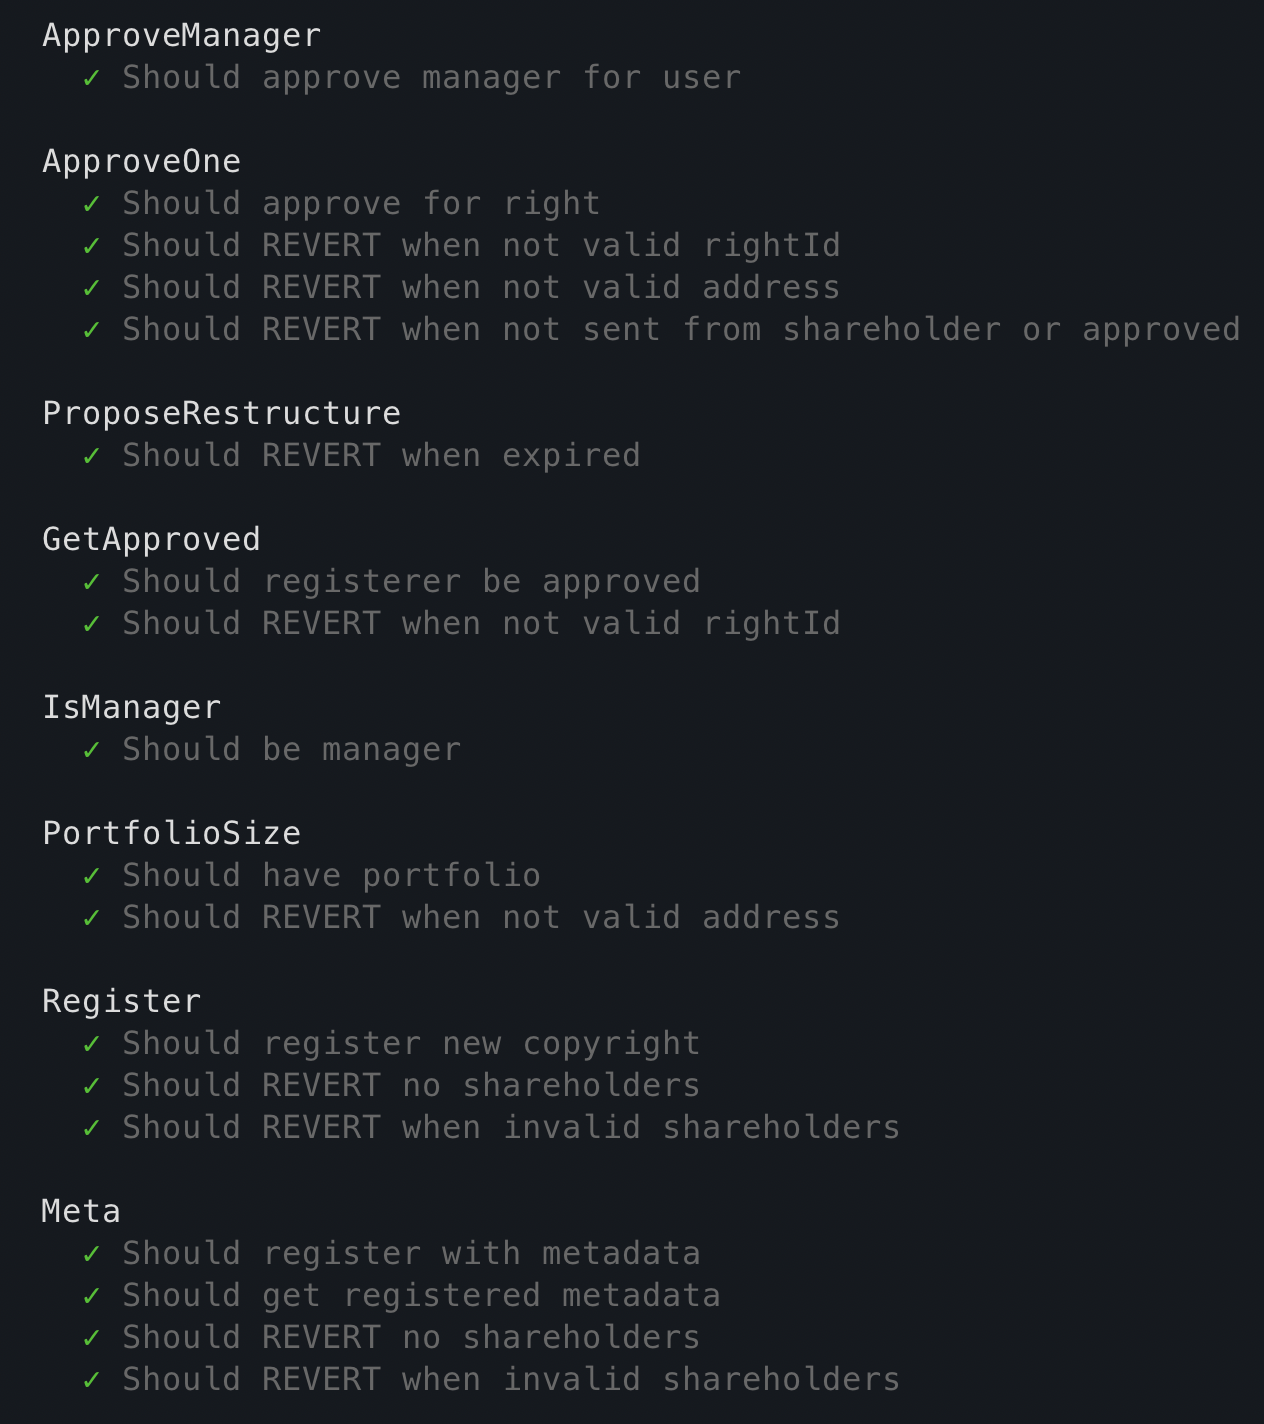
\includegraphics[width=0.7\textwidth,height=\textheight,keepaspectratio]{images/appendix/tests/hardhat-1}
\vfill
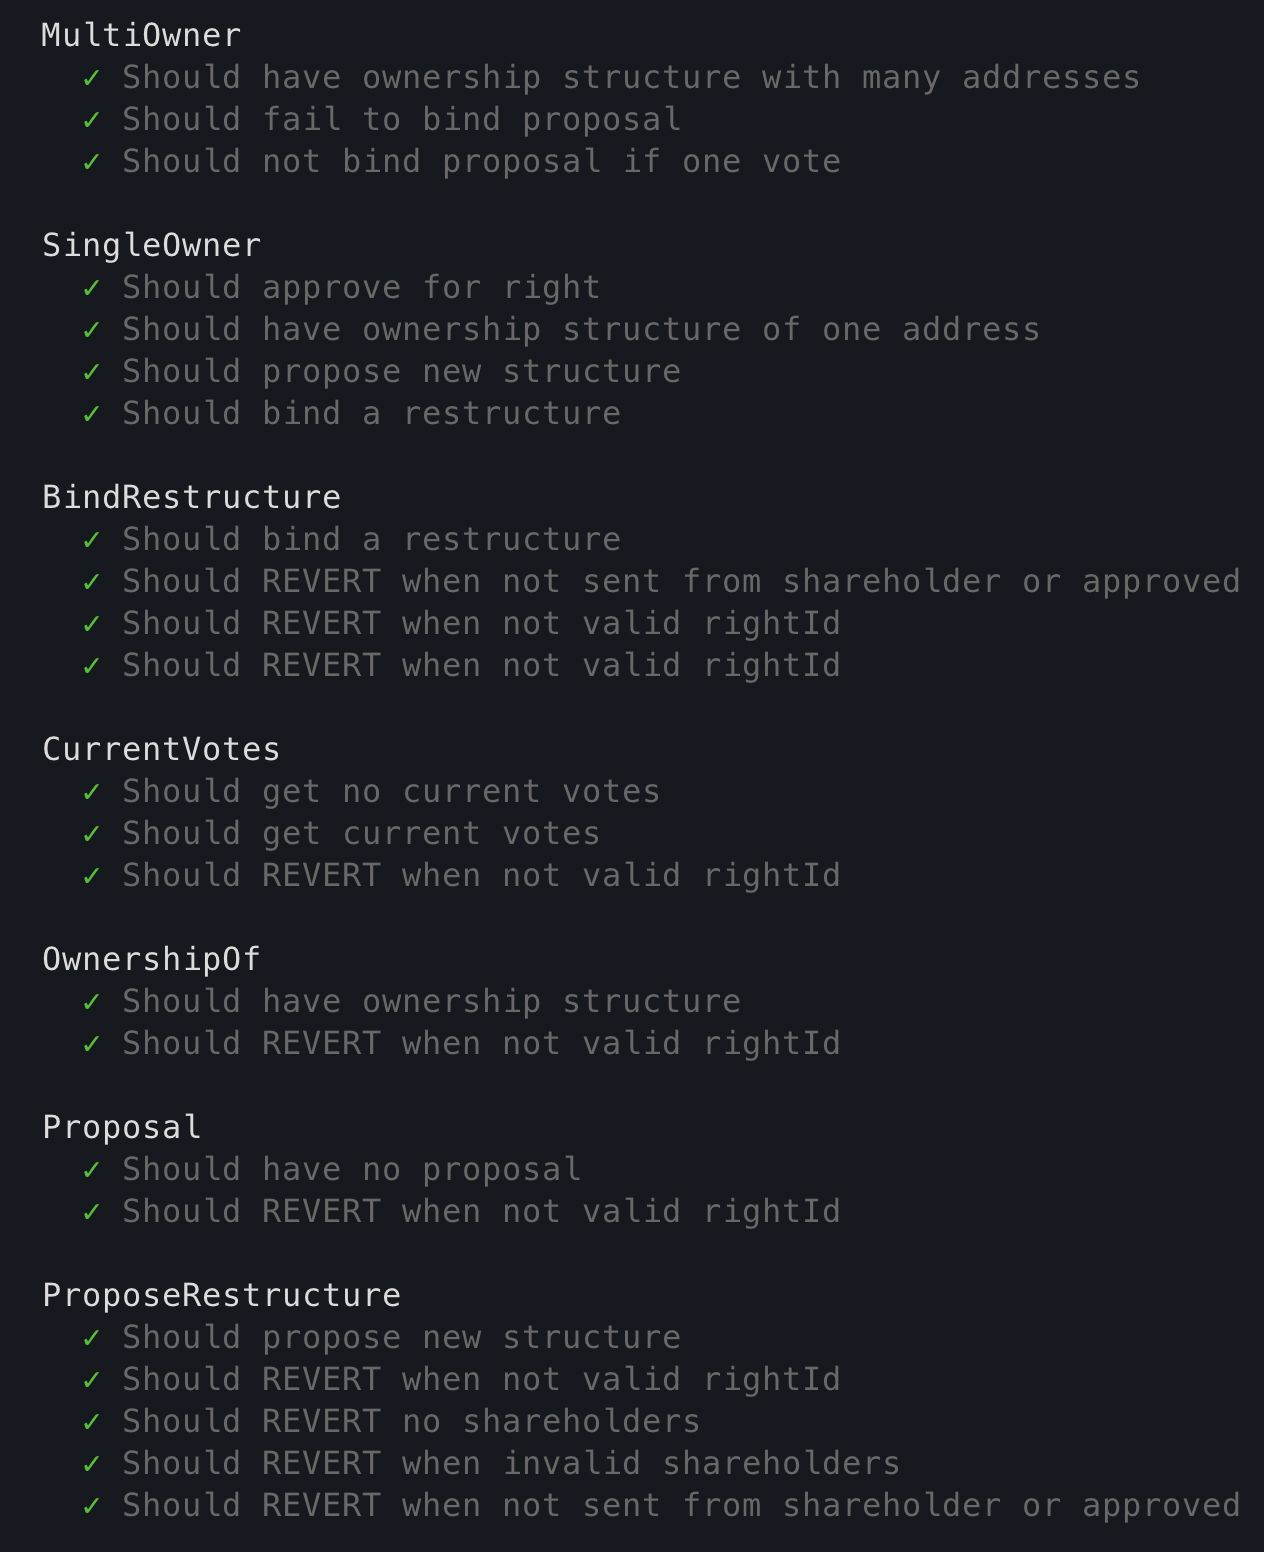
\includegraphics[width=0.7\textwidth,height=\textheight,keepaspectratio]{images/appendix/tests/hardhat-2}

\subsubsection{Back-end unit test results}
\label{sec:test-results:back}

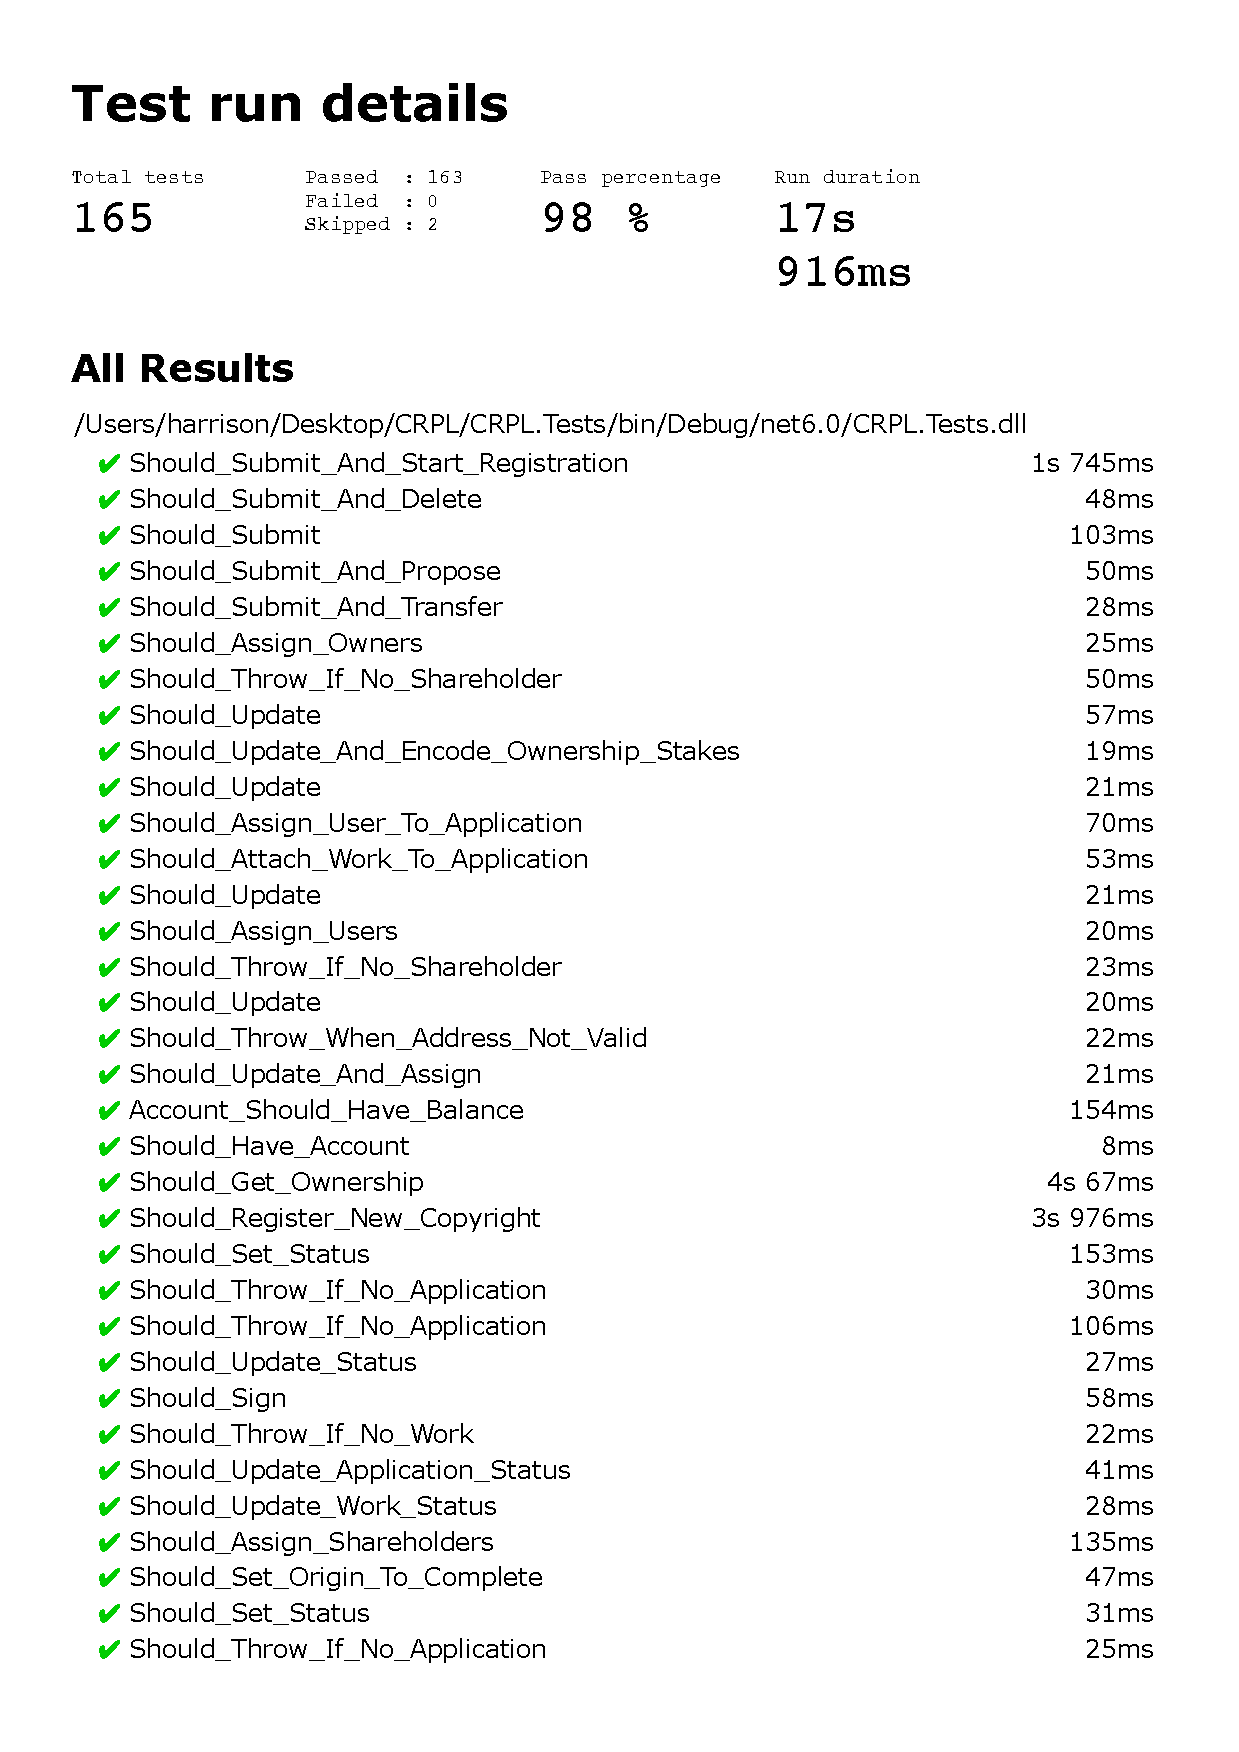
\includepdf[pages=-]{./images/appendix/tests/Back-end-Unit-results.pdf}

\subsubsection{Front-end unit test results}
\label{sec:test-results:front}

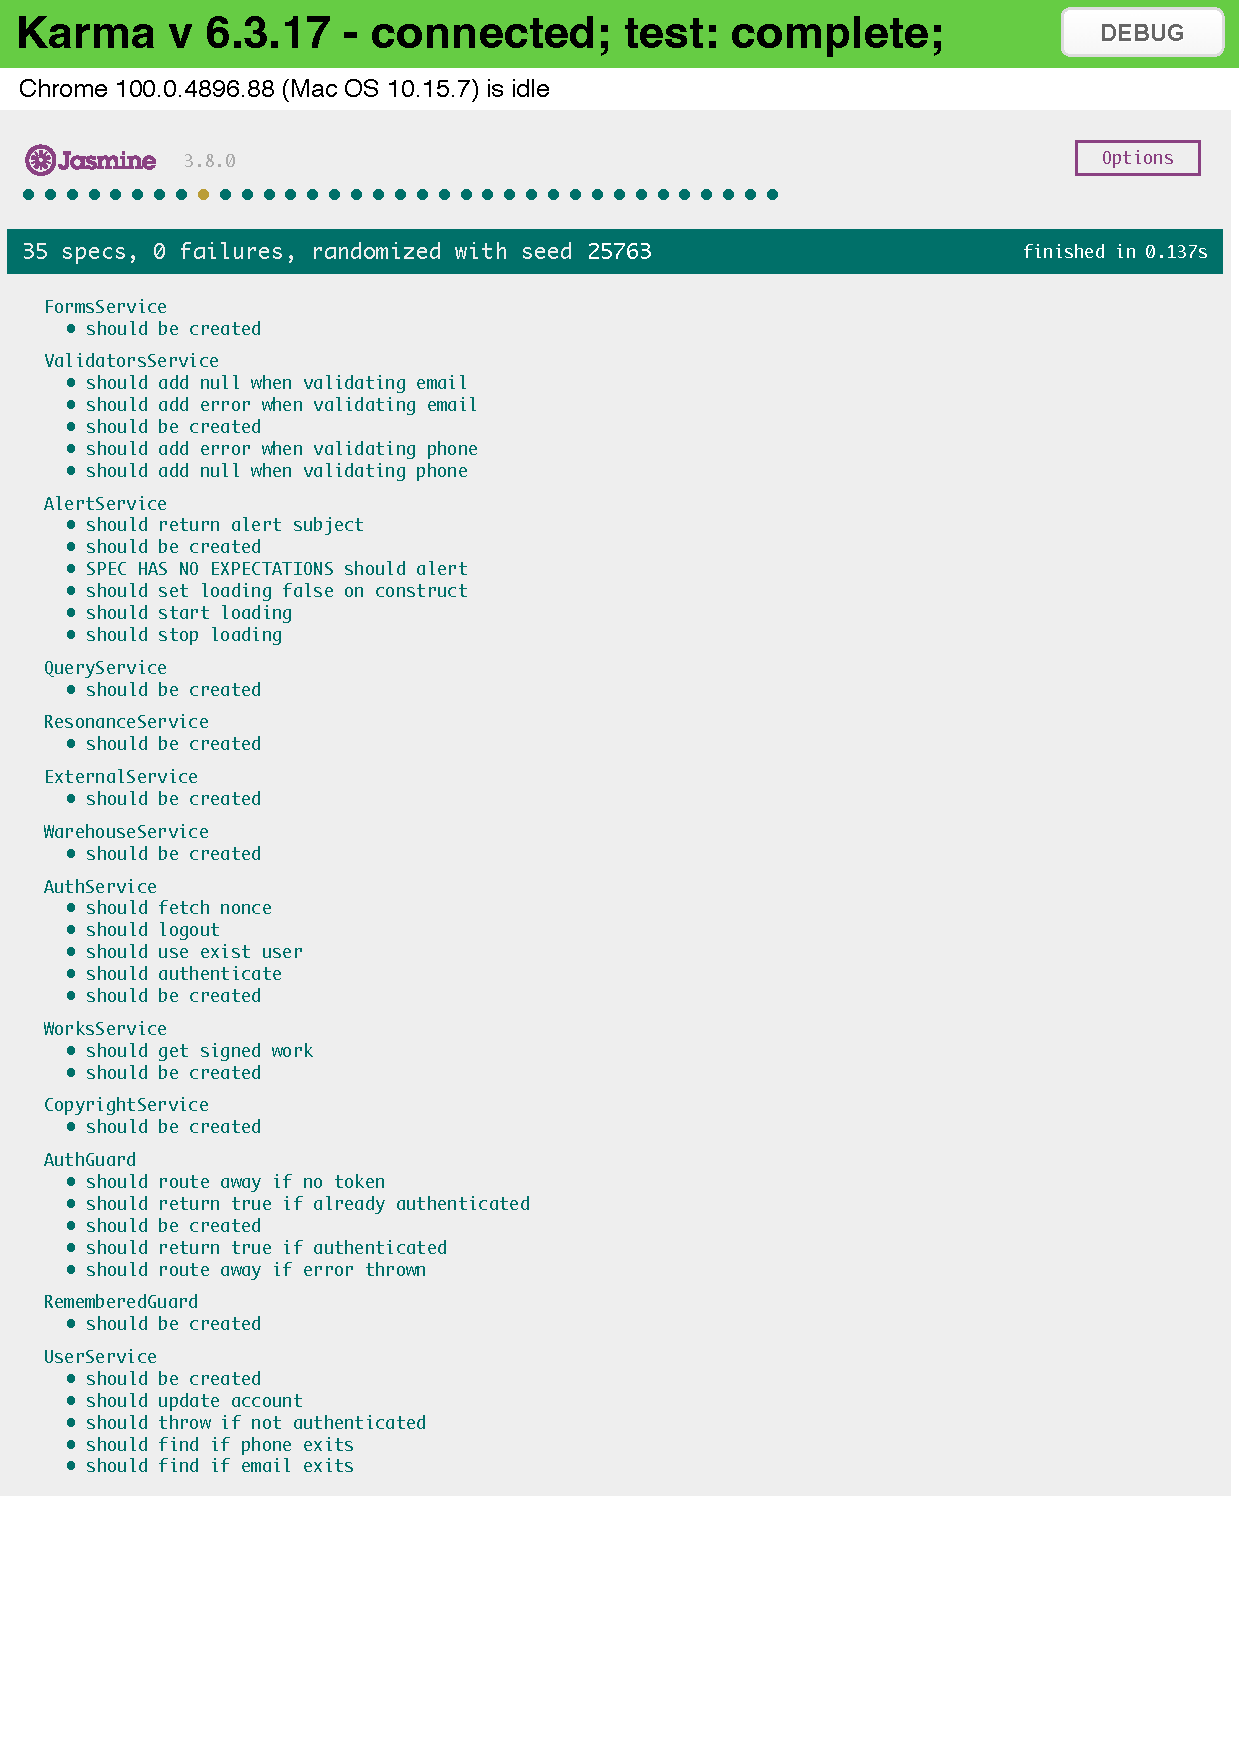
\includepdf[pages=-]{./images/appendix/tests/angular-test-results.pdf}
